\documentclass[11pt,aspectratio=169,handout]{beamer}

\usepackage[utf8]{inputenc}
\usepackage[russian]{babel}
\usepackage{amsmath}
\usepackage{amsfonts}
\usepackage{amssymb}
\usepackage{graphicx}
\usepackage{bibentry}
\usepackage{wasysym}
\usepackage[most]{tcolorbox}
\usepackage[normalem]{ulem}

\usepackage{hyperref}

\usepackage{fontspec}
\setsansfont{VK Sans Display}

\definecolor{info}{RGB}{62, 180, 137}
\definecolor{warn}{RGB}{128, 0, 0}
\definecolor{vk}{RGB}{51, 117, 246}

\useinnertheme{circles}

\setbeamercolor{frametitle}{fg=vk}
\setbeamerfont{frametitle}{size=\LARGE}
\addtobeamertemplate{frametitle}{\vspace*{0.5em}\hspace*{1em}}

\newcommand{\vkitem}{\item[\color{vk}$\bullet$]}

\author{Николай Анохин}
\title{Рекомендательные системы}
\subtitle{и кто над ними работает}

\begin{document}

{
\usebackgroundtemplate{
\includegraphics[width=\paperwidth]{images/title.png}}
\begin{frame}[plain]
\end{frame}
}

\begin{frame}{Обо мне}

\begin{center}
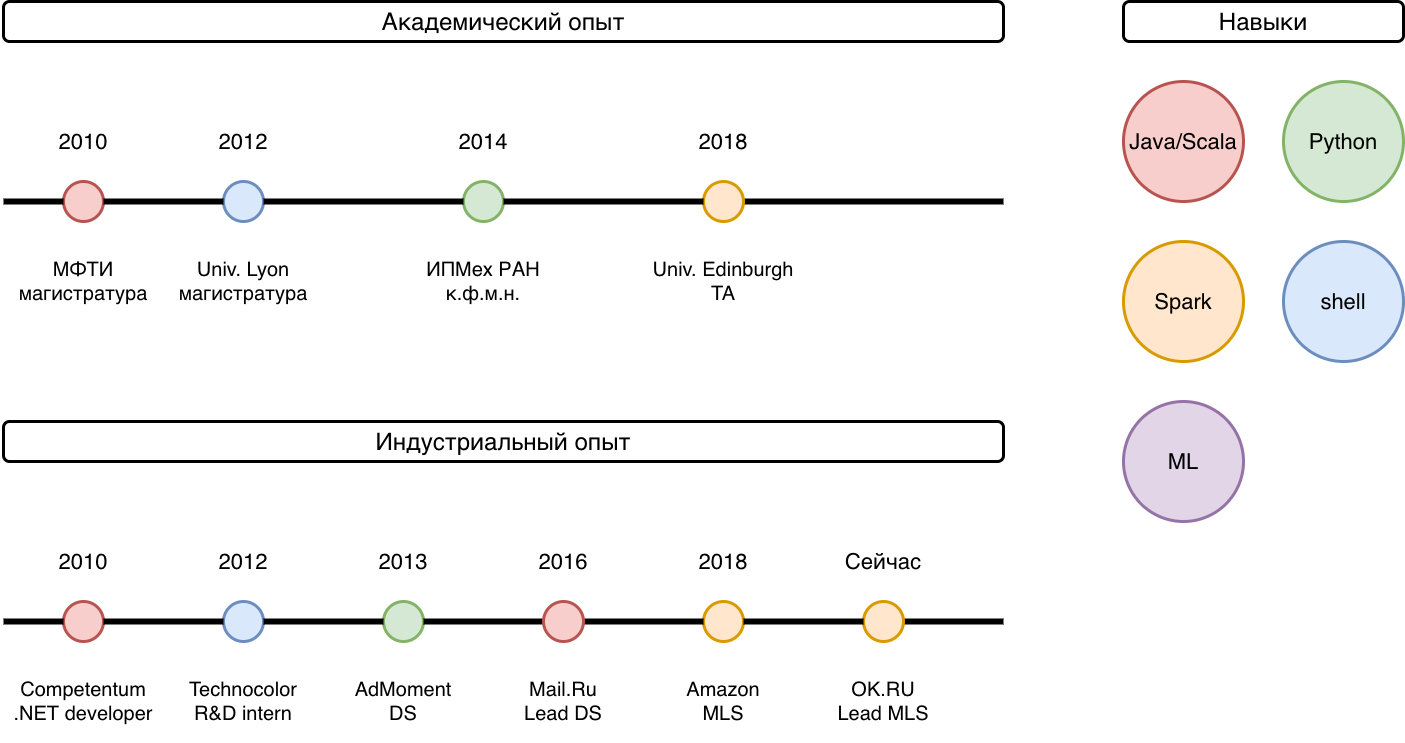
\includegraphics[scale=0.23]{images/about-me.png}
\end{center}

\end{frame}

\begin{frame}{Из этой лекции вы узнаете}

\begin{columns}

\begin{column}{0.58\textwidth}
\begin{itemize}
\vkitem Как устроена рекомендательная система (на примере рекомендаций музыки)
\vkitem Что нужно знать и уметь, чтобы ее создать (это сложно, но вам точно по силам)
\end{itemize}
\end{column}

\begin{column}{0.38\textwidth}
\begin{center}

\includegraphics[scale=0.2]{images/plan.jpeg}
\end{center}
\end{column}

\end{columns}

\end{frame}

\begin{frame}{Зачем нужны рекомендательные системы \cite{RSHB}}

\begin{columns}

\begin{column}{0.4\textwidth}

\includegraphics[scale=0.25]{images/logos.png}
\end{column}

\pause

\begin{column}{0.5\textwidth}

\begin{itemize}[<+->]

\vkitem {\bf Бизнесу}
\begin{itemize}
\vkitem Увеличить продажи
\vkitem Добиться большей лояльности
\vkitem Улучшить пользовательский опыт
\end{itemize}

\vkitem {\bf Пользователям}
\begin{itemize}
\vkitem Найти лучший товар
\vkitem Найти {\bf все} подходящие товары
\vkitem Залипнуть
\end{itemize}

\end{itemize}

\end{column}

\end{columns}

\end{frame}

{
\usebackgroundtemplate{\includegraphics[width=\paperwidth, height=\paperheight]{images/netflix-0.png}}
\begin{frame}[plain]
\end{frame}
}

{
\usebackgroundtemplate{\includegraphics[width=\paperwidth, height=\paperheight]{images/netflix-1.png}}
\begin{frame}[plain]
\end{frame}
}

{
\usebackgroundtemplate{\includegraphics[width=\paperwidth, height=\paperheight]{images/netflix-2.png}}
\begin{frame}[plain]
\end{frame}
}

{
\usebackgroundtemplate{\includegraphics[width=\paperwidth, height=\paperheight]{images/netflix-3.png}}
\begin{frame}[plain]
\end{frame}
}

{
\usebackgroundtemplate{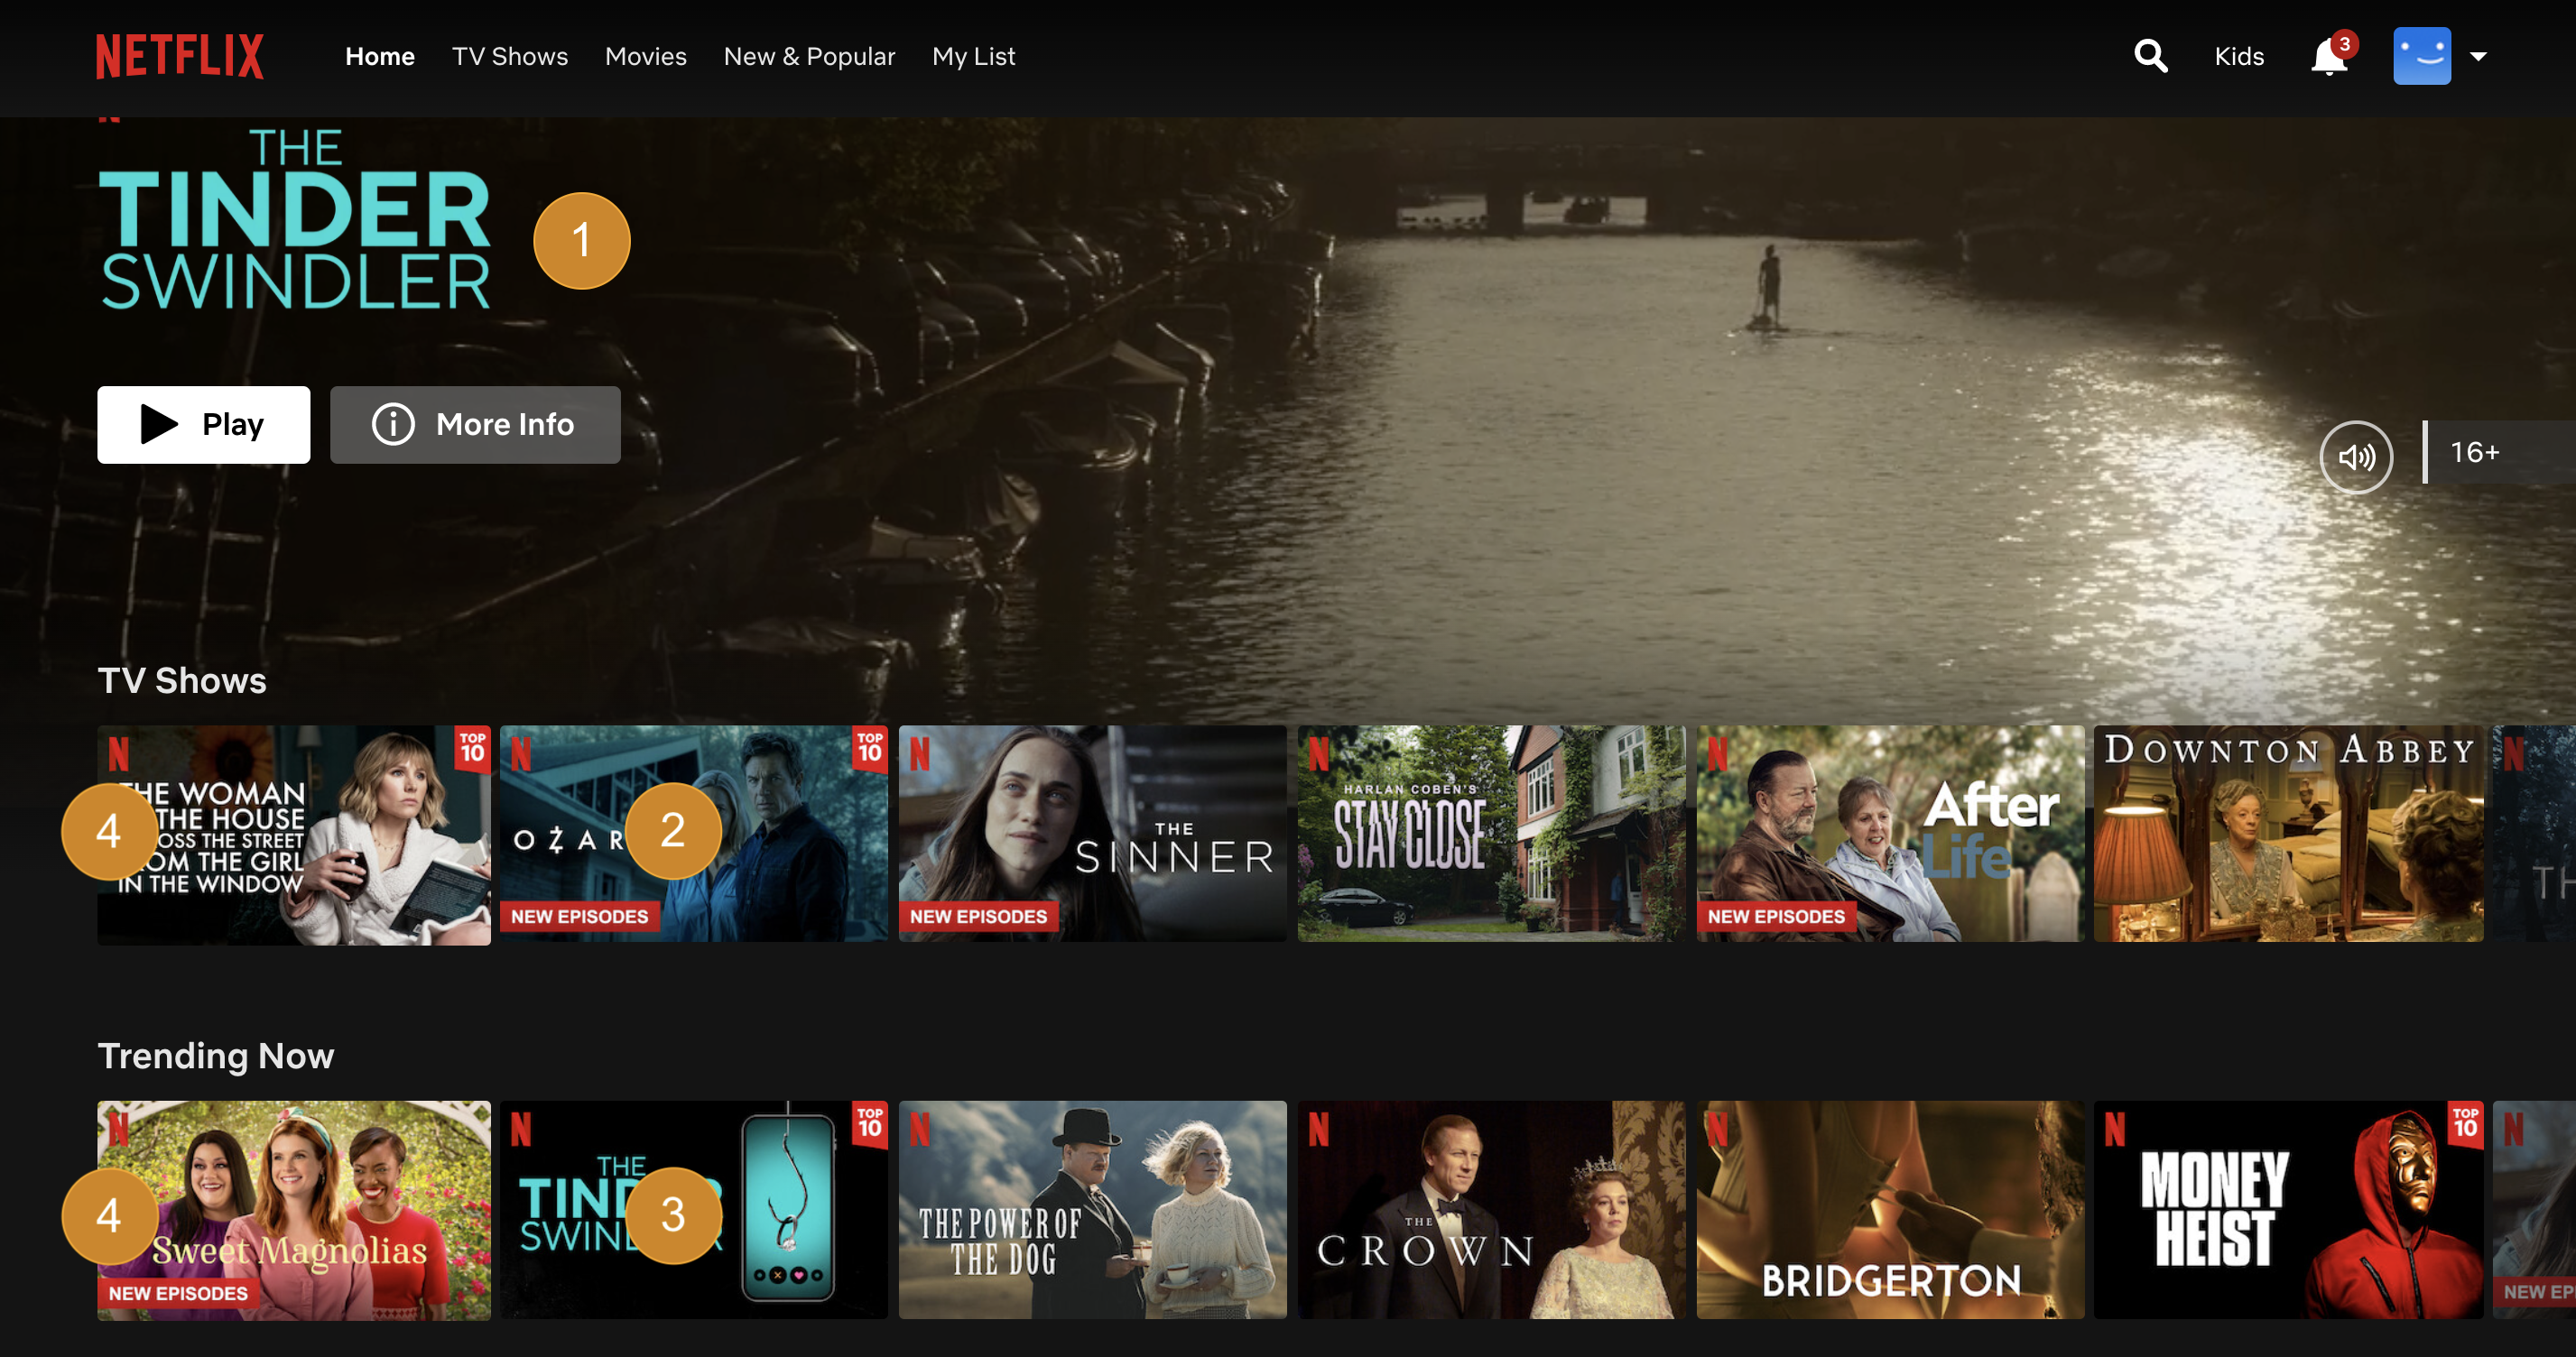
\includegraphics[width=\paperwidth, height=\paperheight]{images/netflix-4.png}}
\begin{frame}[plain]
\end{frame}
}

{
\usebackgroundtemplate{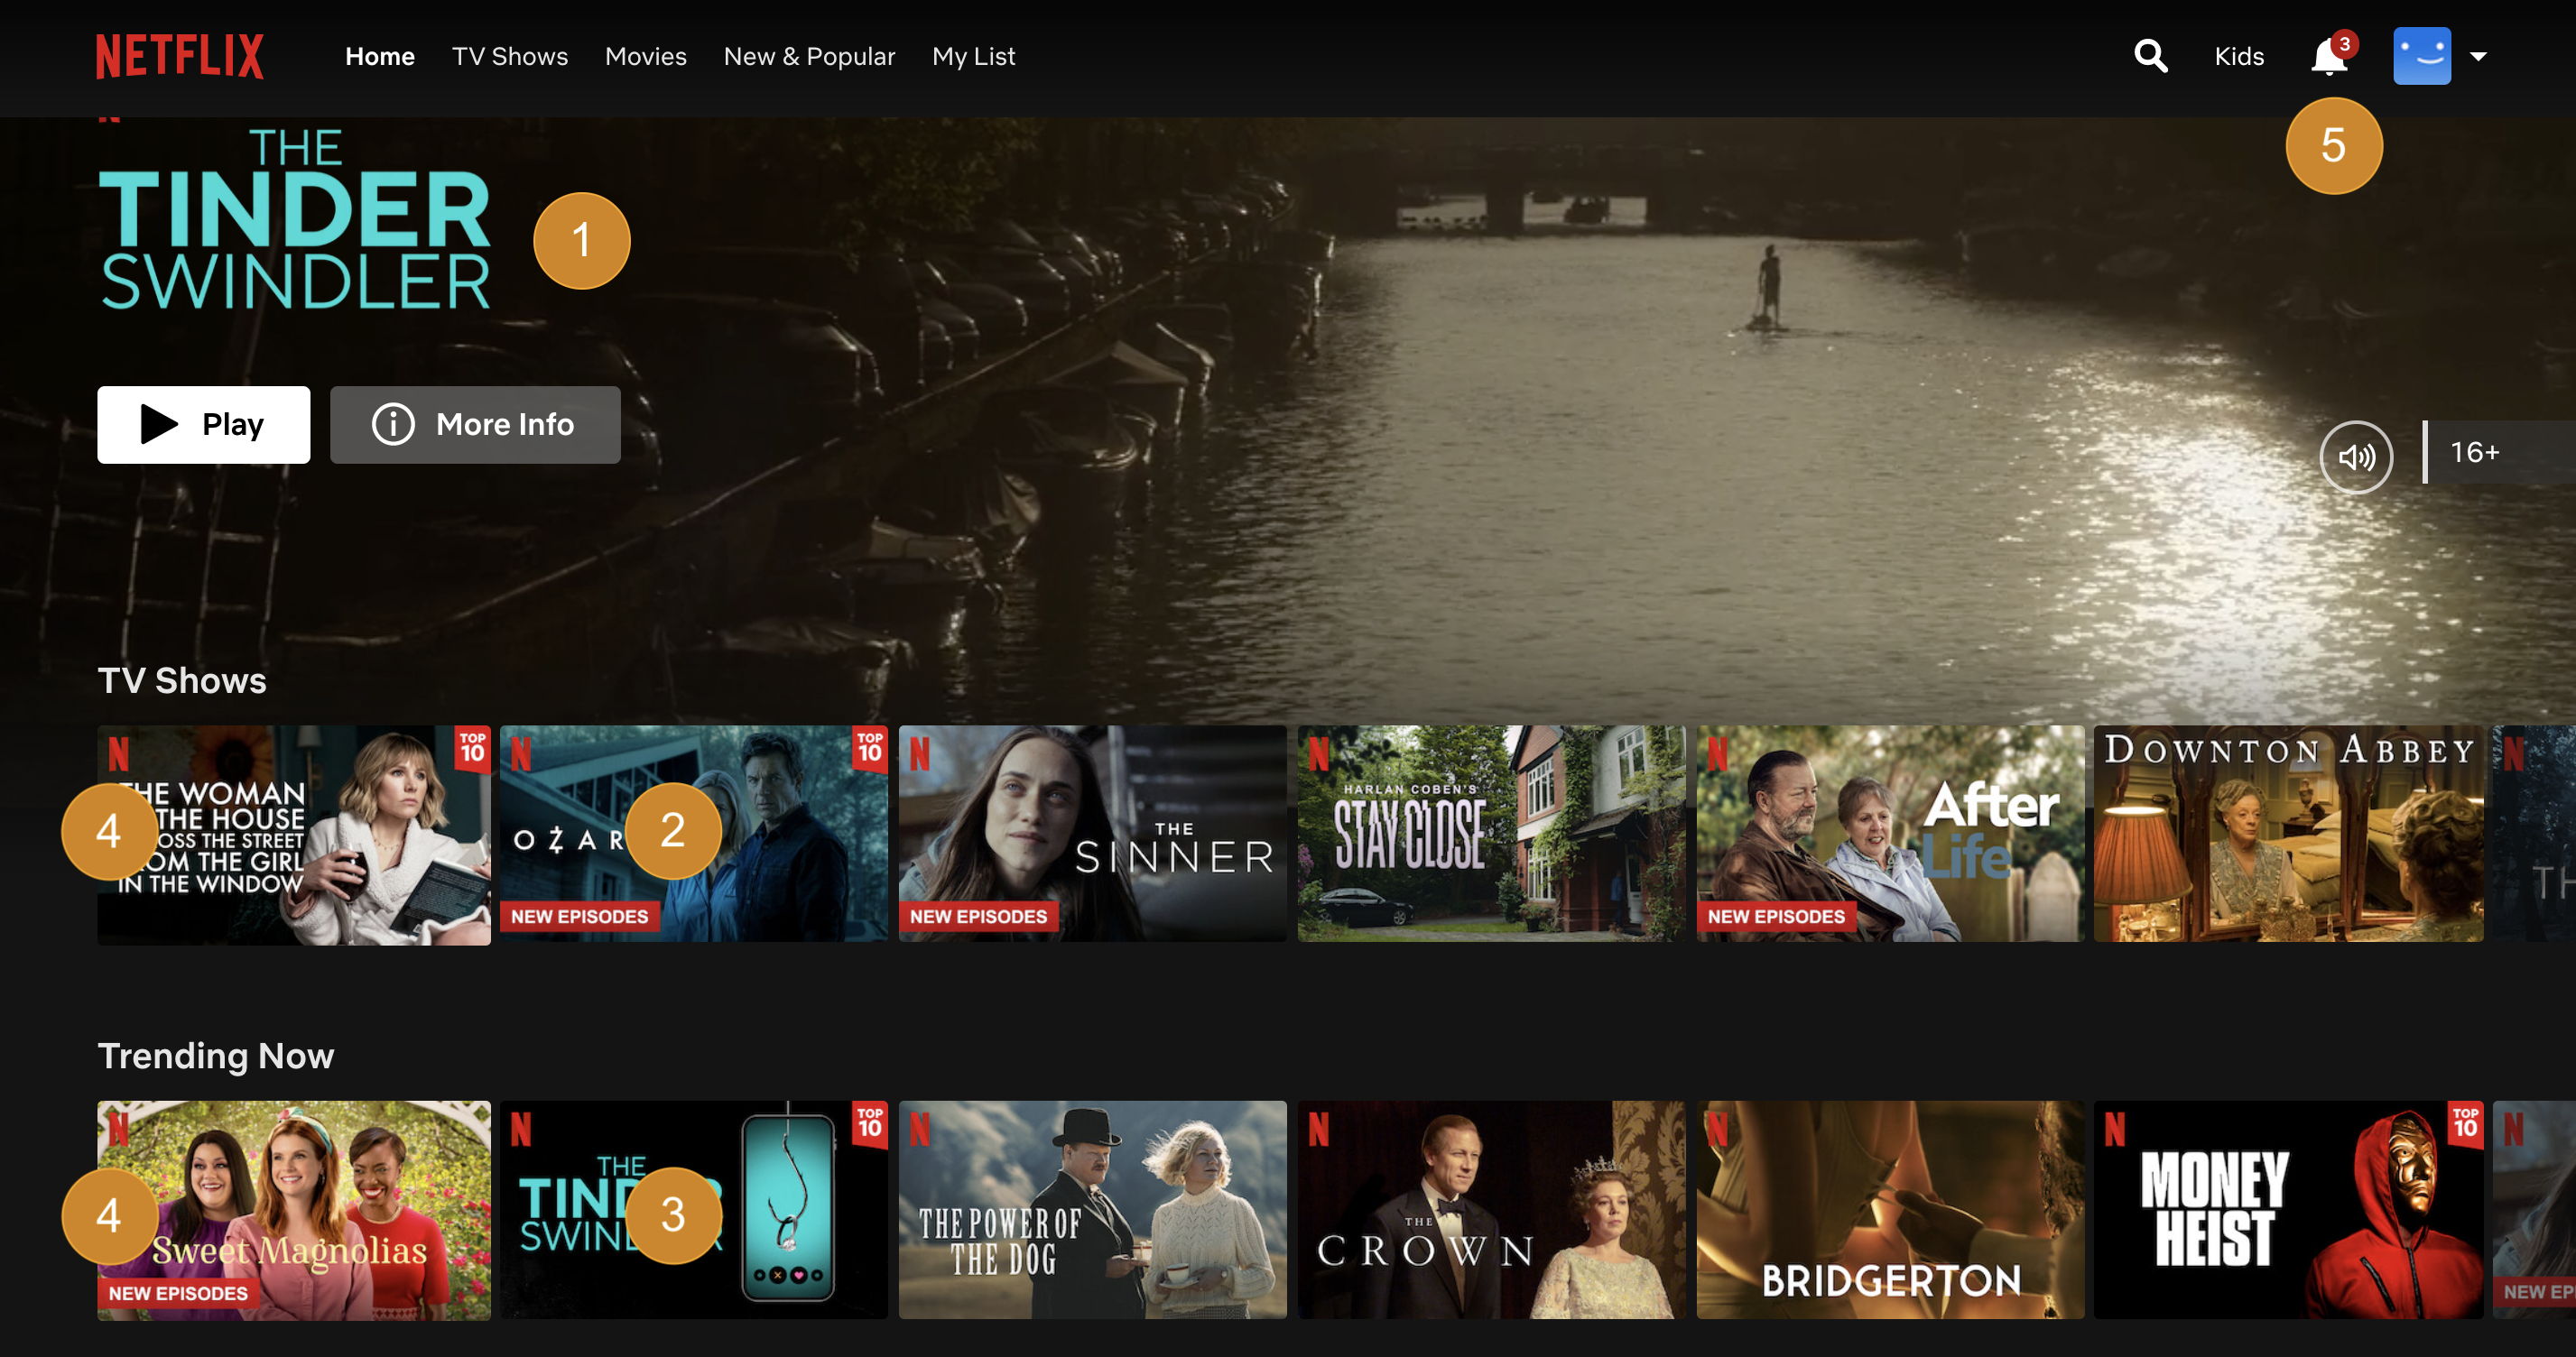
\includegraphics[width=\paperwidth, height=\paperheight]{images/netflix-5.png}}
\begin{frame}[plain]
\end{frame}
}

{
\usebackgroundtemplate{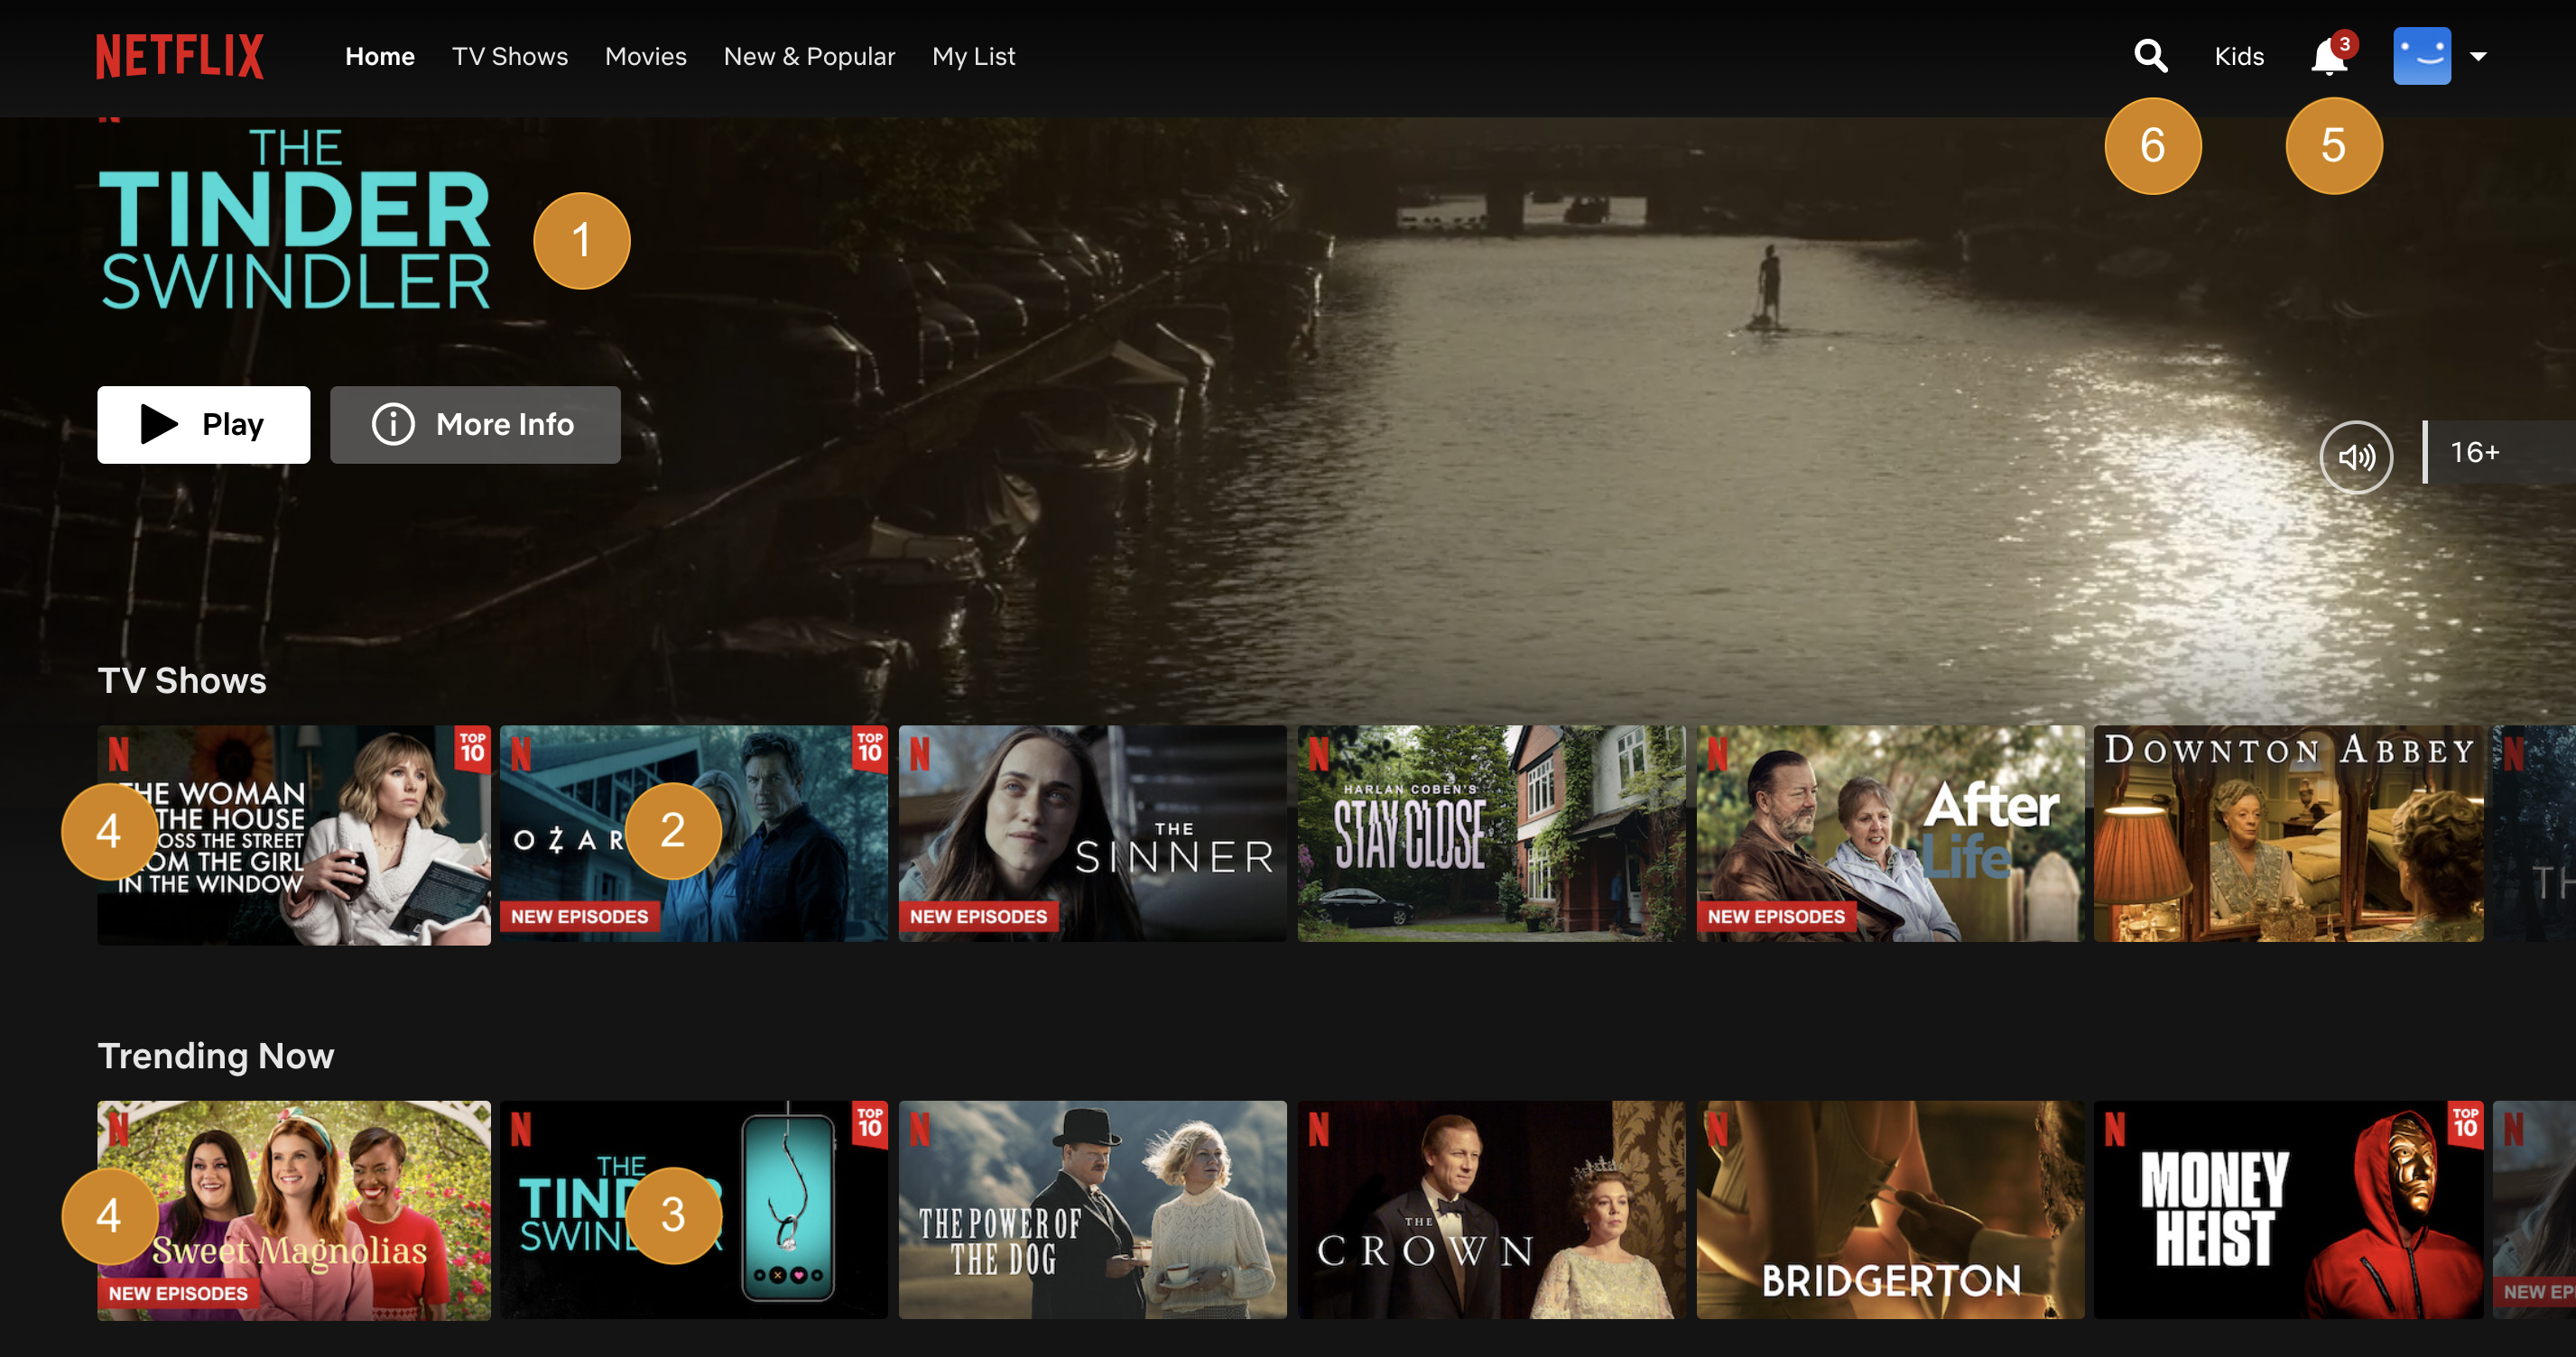
\includegraphics[width=\paperwidth, height=\paperheight]{images/netflix-6.png}}
\begin{frame}[plain]
\end{frame}
}

\begin{frame}{Рекомендации музыки}

\begin{columns}
\begin{column}{0.55\textwidth}
   {\bf Задача} \\
   Рекомендовать пользователю {\bf исполнителей}, так чтобы пользователь слушал их песни и {\bf как можно дольше} оставался в приложении
\end{column}
\begin{column}{0.3\textwidth}
    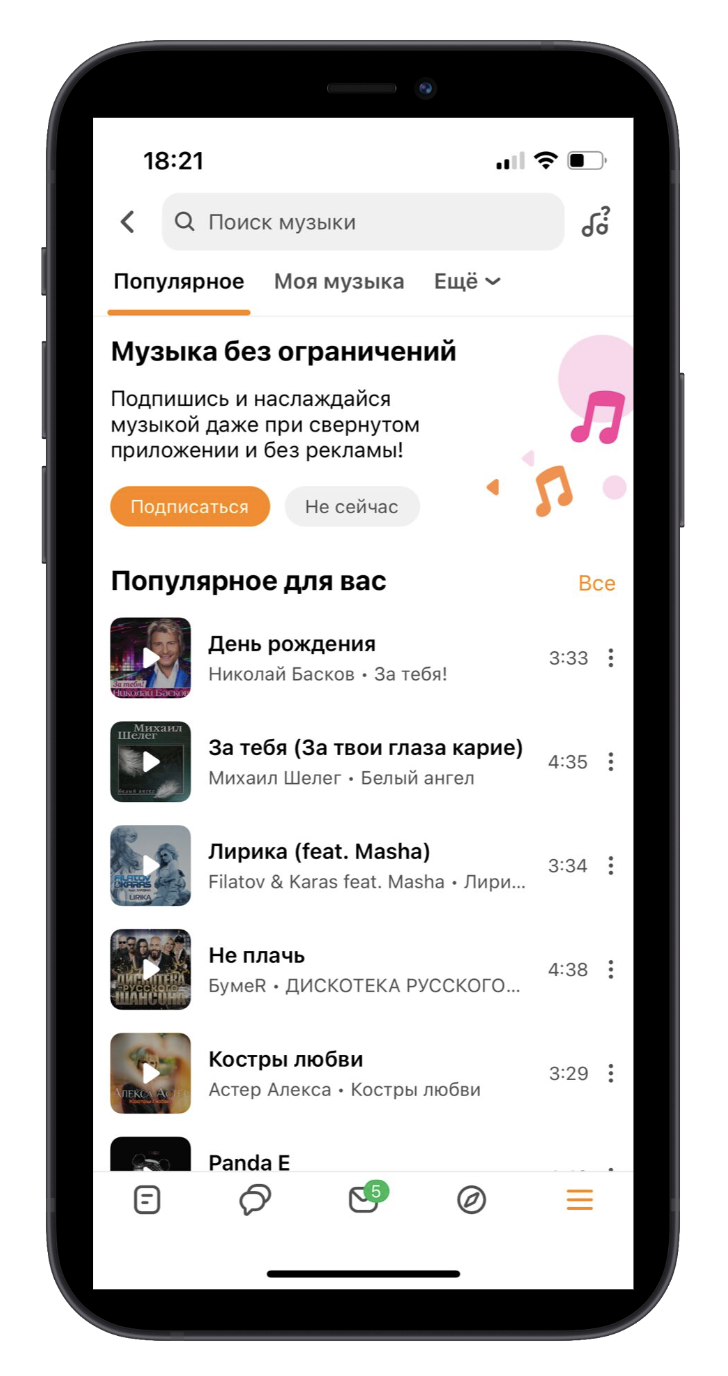
\includegraphics[scale=0.25]{images/music-screen.png}
\end{column}
\end{columns}

\end{frame}

\section{Алгоритм рекомендаций}

{
\usebackgroundtemplate{
\includegraphics[width=\paperwidth]{images/part-1.png}}
\begin{frame}[plain]
\end{frame}
}

\begin{frame}{Как строить рекомендации}

\begin{center}

\begin{center}
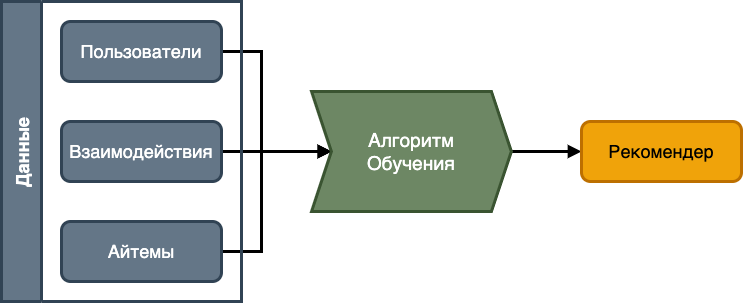
\includegraphics[scale=0.35]{images/learning.png}
\end{center}

\end{center}

\end{frame}

\begin{frame}{Зоопарк алгоритмов рекомендаций \cite{ali_2021}}

\begin{center}
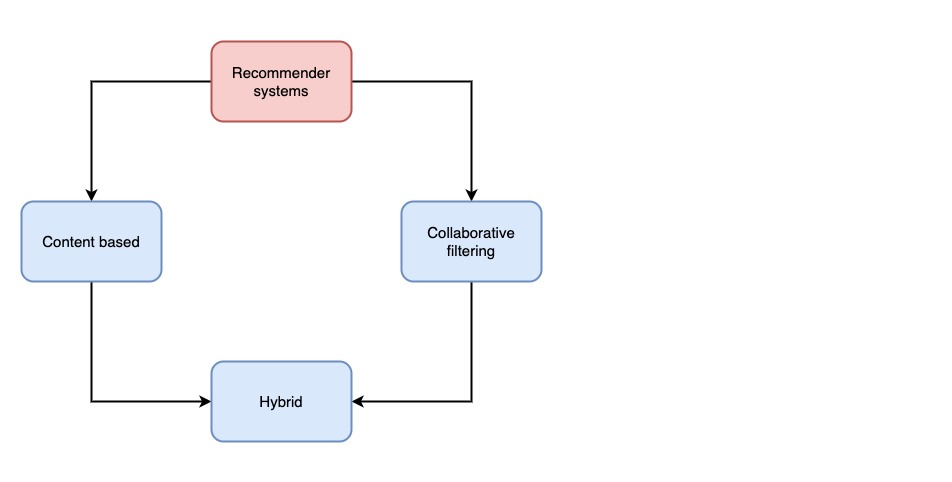
\includegraphics[scale=0.27]{images/taxonomy-1.png}
\end{center}


\includegraphics[scale=0.3]{images/poll.png} \hfill \url{http://shorturl.at/foqB7}

\end{frame}

\begin{frame}{Зоопарк алгоритмов рекомендаций \cite{ali_2021}}

\begin{center}
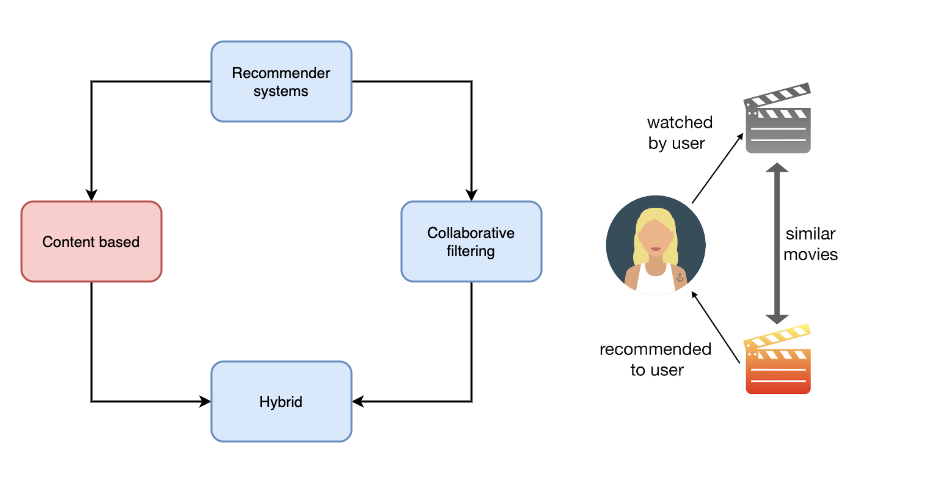
\includegraphics[scale=0.27]{images/taxonomy-2.png}
\end{center}


\includegraphics[scale=0.3]{images/poll.png} \hfill \url{http://shorturl.at/foqB7}

\end{frame}

\begin{frame}{Зоопарк алгоритмов рекомендаций \cite{ali_2021}}

\begin{center}
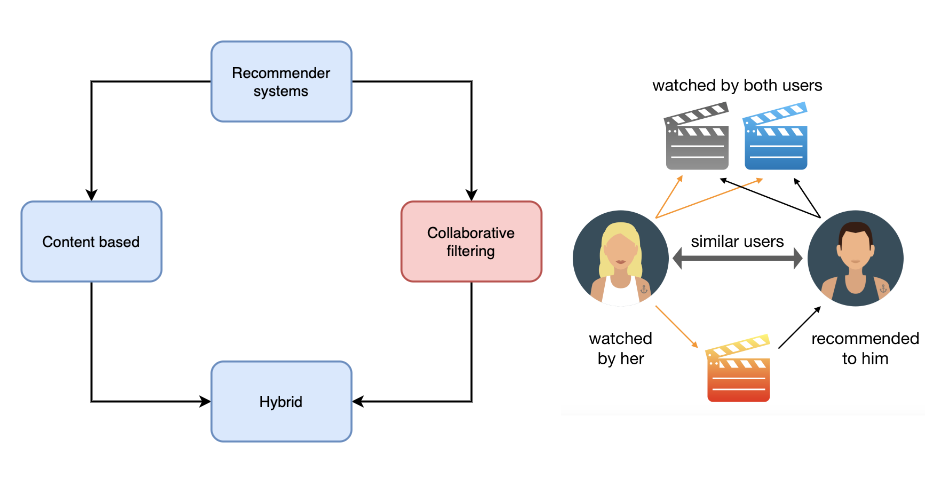
\includegraphics[scale=0.27]{images/taxonomy-3.png}
\end{center}


\includegraphics[scale=0.3]{images/poll.png} \hfill \url{http://shorturl.at/foqB7}

\end{frame}

\begin{frame}{Зоопарк алгоритмов рекомендаций \cite{ali_2021}}

\begin{center}
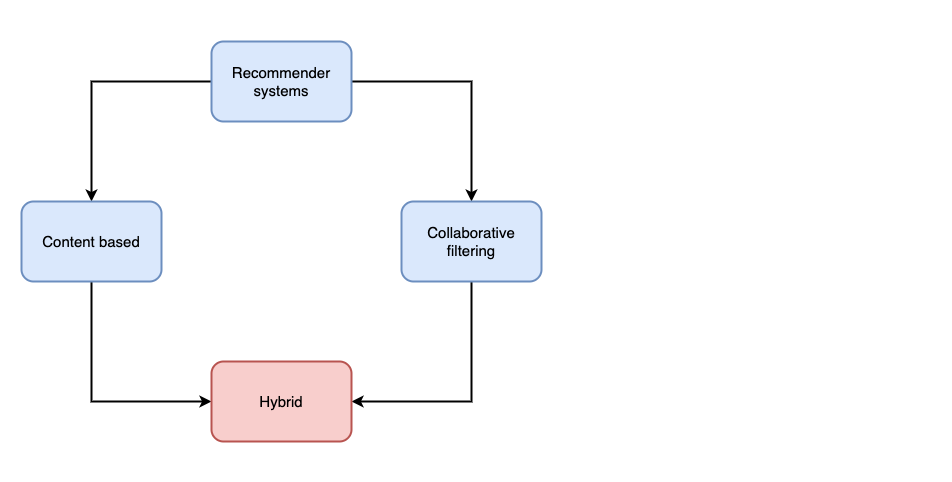
\includegraphics[scale=0.27]{images/taxonomy-4.png}
\end{center}


\includegraphics[scale=0.3]{images/poll.png} \hfill \url{http://shorturl.at/foqB7}

\end{frame}

\begin{frame}{}

\begin{center}

\includegraphics[scale=0.4]{images/compile.png}
\end{center}

\end{frame}

\begin{frame}{Personalized Page Rank (PPR) \cite{PPR}}

\begin{columns}
\begin{column}{0.4\textwidth}
\begin{center}
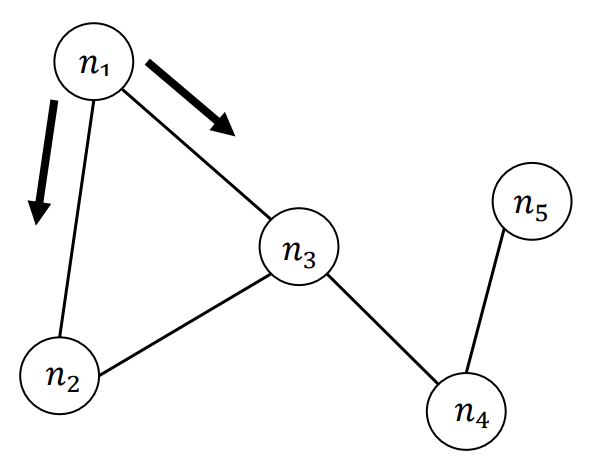
\includegraphics[scale=0.4]{images/example-graph.png}
\end{center}
\end{column}

\begin{column}{0.5\textwidth}
\begin{footnotesize}
Начальное состояние
\[
\vec{s}_0 = \begin{pmatrix}
	1 & 0 & 0 & 0 & 0
\end{pmatrix}
\]

Вероятность перехода
\[
\vec{p}_{n+1} = c \vec{s}_n \cdot P + (1 - c) \vec{s}_0 
\]
\[
P = \begin{pmatrix}
	0 & 1/2 & 1/2 & 0 & 0 \\
	1/2 & 0 & 1/2 & 0 & 0 \\
	1/3 & 1/3 & 0 & 1/3 & 0 \\
	0 & 0 & 1/2 & 0 & 1/2 \\
	0 & 0 & 0 & 1 & 0
\end{pmatrix}
\]
$(1-c)$ -- вероятность рестарта
\end{footnotesize}
\end{column}

\end{columns}

\begin{tcolorbox}[colback=vk!5,colframe=vk!70,title=]
Где мы окажемся через бесконечное число шагов?
\end{tcolorbox}

\end{frame}

\begin{frame}{Строим граф исполнителей: создаем ребра I}

Коля: Лепс, Газманов, Adele

\pause

\begin{center}
\begin{tcolorbox}[colback=vk!5,colframe=vk!70,title=Задача]
Есть $K$ пользователей. Пользователь $j$ случайным образом с равной вероятностью без возвращения выбирает $n_j$ из $N$ исполнителей. Сколько в среднем пользователей выберут каждую пару исполнителей? 
\end{tcolorbox}
\end{center}

\pause

{\bf Ответ}
\[
E_1 + \ldots + E_K = \frac{\sum_{j=1}^K n_j (n_j - 1)}{N (N-1)}
\]
	
\end{frame}

\begin{frame}{Строим граф исполнителей: создаем ребра II}

\begin{center}
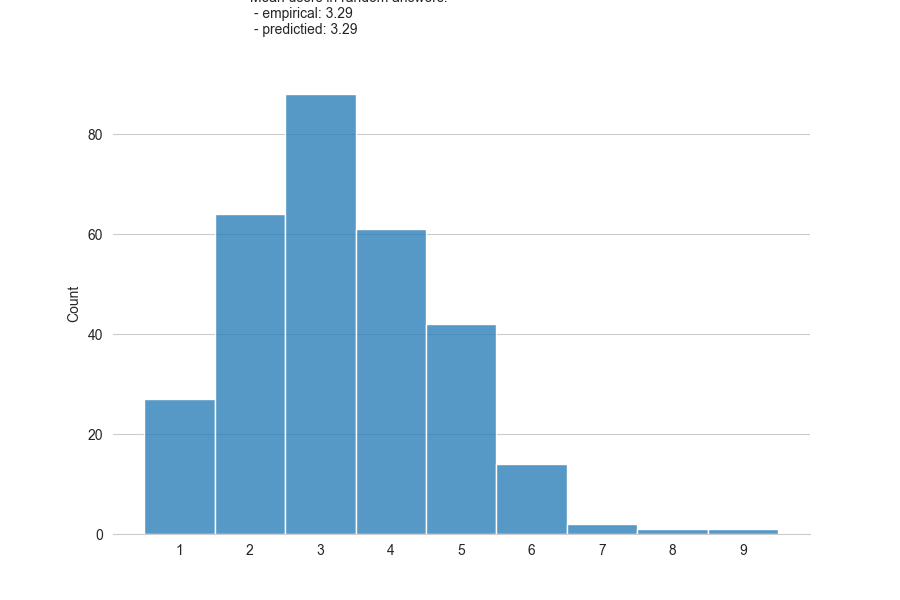
\includegraphics[scale=0.4]{images/user_counts.png}
\end{center}

\end{frame}

\begin{frame}{Строим граф исполнителей III}

\begin{center}
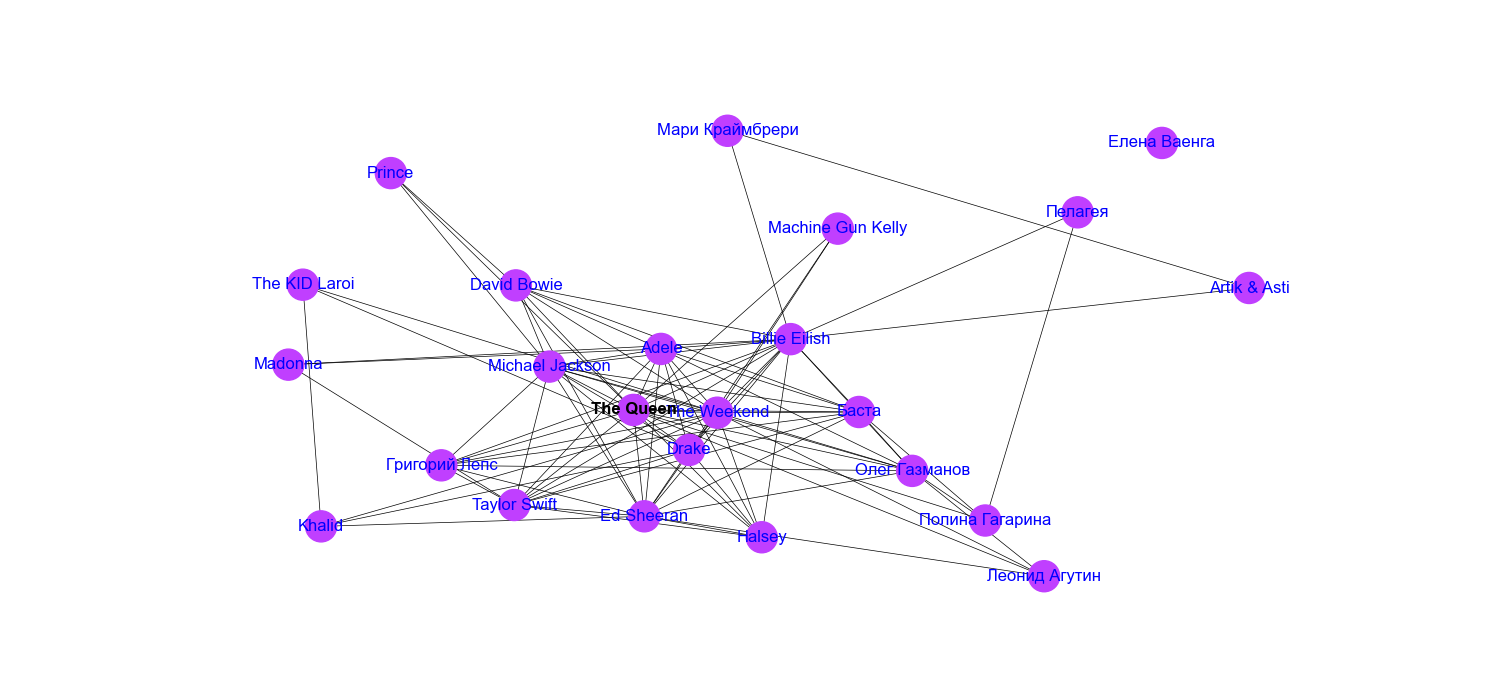
\includegraphics[scale=0.35]{images/graph.png}
\end{center}

\end{frame}

\begin{frame}{Cлучайные блуждания по графу исполнителей}

\href{http://localhost:8888/lab/workspaces/auto-u/tree/images/random_walk.gif}{\color{blue}Ссылка на визуализацию}

\end{frame}

\begin{frame}{Рекомендации на основе блужданий}

\begin{center}
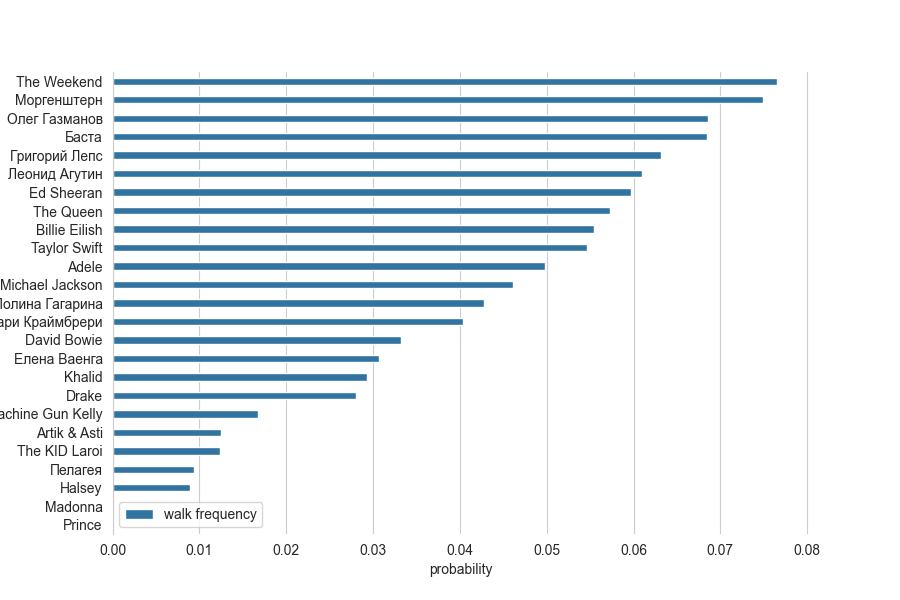
\includegraphics[scale=0.4]{images/recommendations-1.png}
\end{center}

\end{frame}

\begin{frame}{Рекомендации на основе точного решения}

\[
\vec{r} = c \vec{r} P + (1 - c) \vec{s} \quad \rightarrow \quad \vec{r} = (1 - c) \vec{s} \left(I - c P \right)^{-1}
\]

\begin{center}
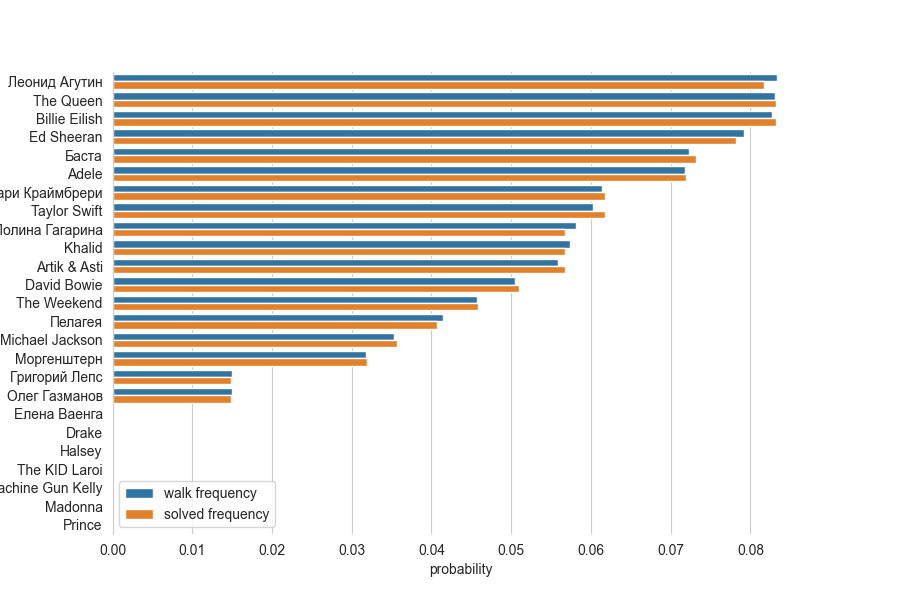
\includegraphics[scale=0.4]{images/recommendations-2.png}
\end{center}

\end{frame}

{
\usebackgroundtemplate{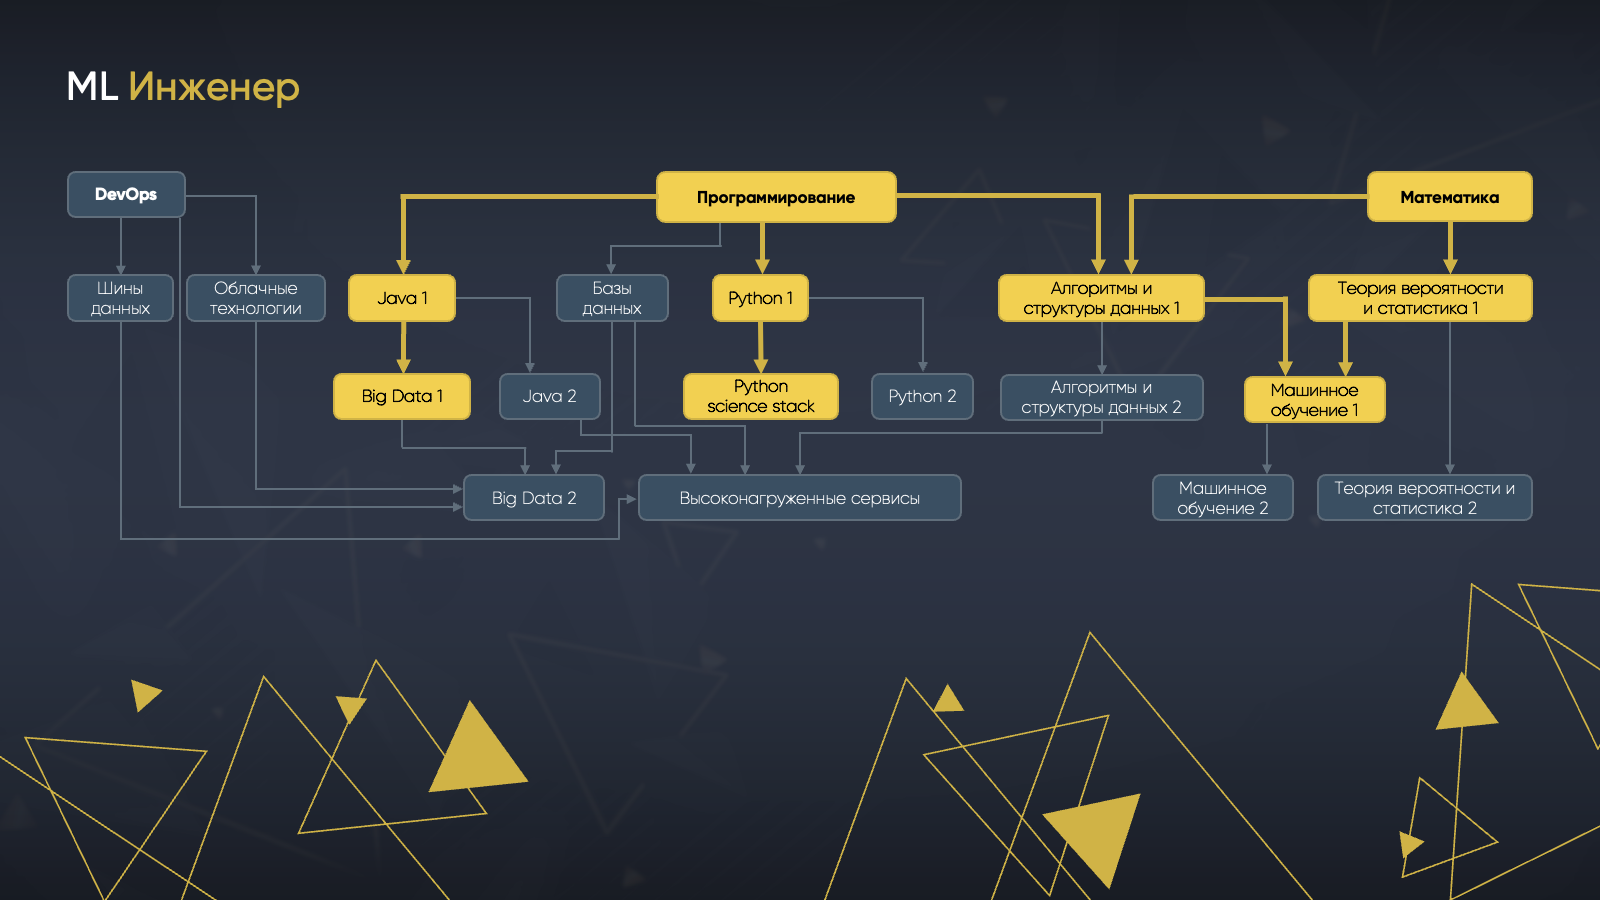
\includegraphics[width=\paperwidth]{images/mle.png}}
\begin{frame}[plain]
\end{frame}
}

\section{Продакшен}

{
\usebackgroundtemplate{
\includegraphics[width=\paperwidth]{images/part-2.png}}
\begin{frame}[plain]
\end{frame}
}

\begin{frame}{Сервис рекомендаций}

\begin{center}
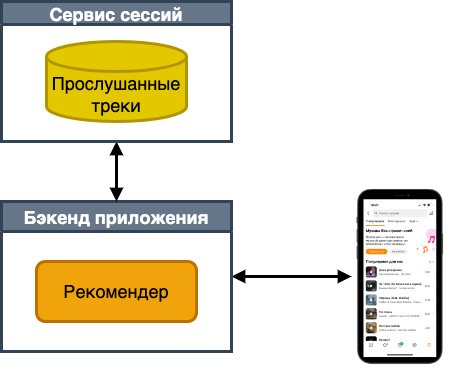
\includegraphics[scale=0.35]{images/backend.png}
\end{center}

\end{frame}

{
\usebackgroundtemplate{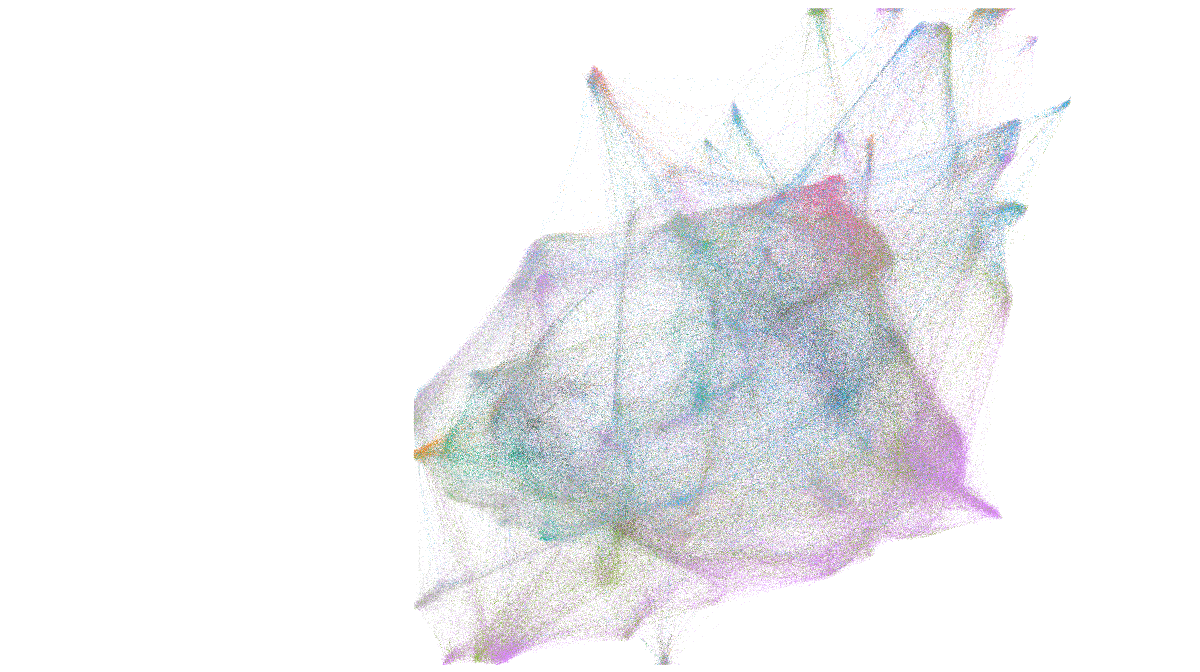
\includegraphics[width=\paperwidth]{images/ok-music-graph.png}}
\begin{frame}[plain]{Граф исполнителей в Одноклассниках}

{\bf Параметры графа}

20000 вершин

750000 ребер 

\pause

\vfill

{\bf Память}

\pause

$O(N_{nodes}^2)$

\vfill

{\bf Сложность}

Прямое решение $\vec{r} = (1 - c) \vec{s} \left(I - c P \right)^{-1}$

\pause

$O(N_{nodes}^3)$

\end{frame}
}

\begin{frame}{Оптимизируем вычисление рекомендаций \cite{PPR}}

\begin{columns}

\begin{column}{0.5\textwidth}
\begin{itemize}[<+->]
\vkitem Сэмплирование монте-карло
\vkitem Оптимизированное прямое решение
\vkitem Оптимизированный power iteration
\end{itemize}
\end{column}

\begin{column}{0.4\textwidth}
\begin{center}
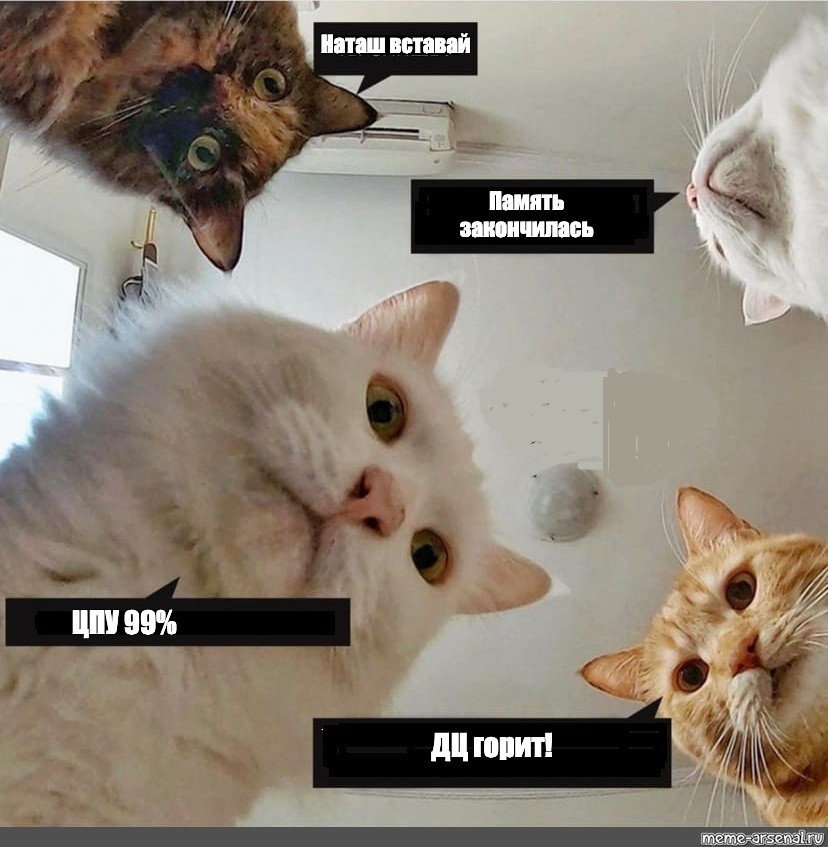
\includegraphics[scale=0.2]{images/natash.jpeg}
\end{center}
\end{column}

\end{columns}

\end{frame}

{
\usebackgroundtemplate{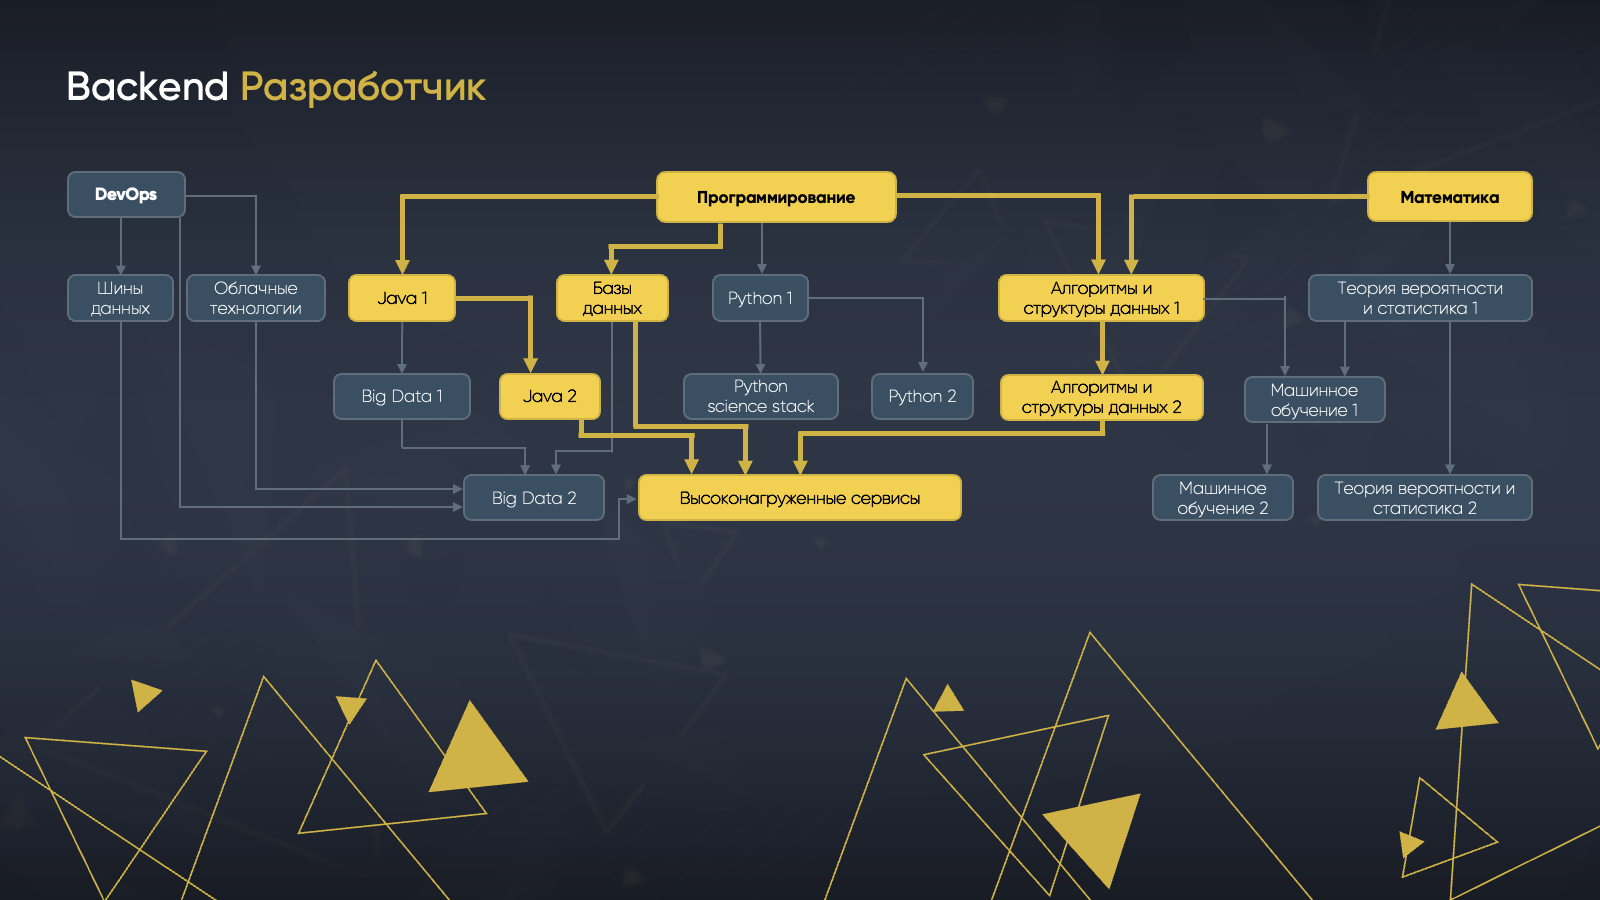
\includegraphics[width=\paperwidth]{images/bed.png}}
\begin{frame}[plain]
\end{frame}
}

\section{Данные для рекомендаций}

{
\usebackgroundtemplate{
\includegraphics[width=\paperwidth]{images/part-3.png}}
\begin{frame}[plain]
\end{frame}
}

\begin{frame}{Транспорт данных между сервисами}

\begin{center}
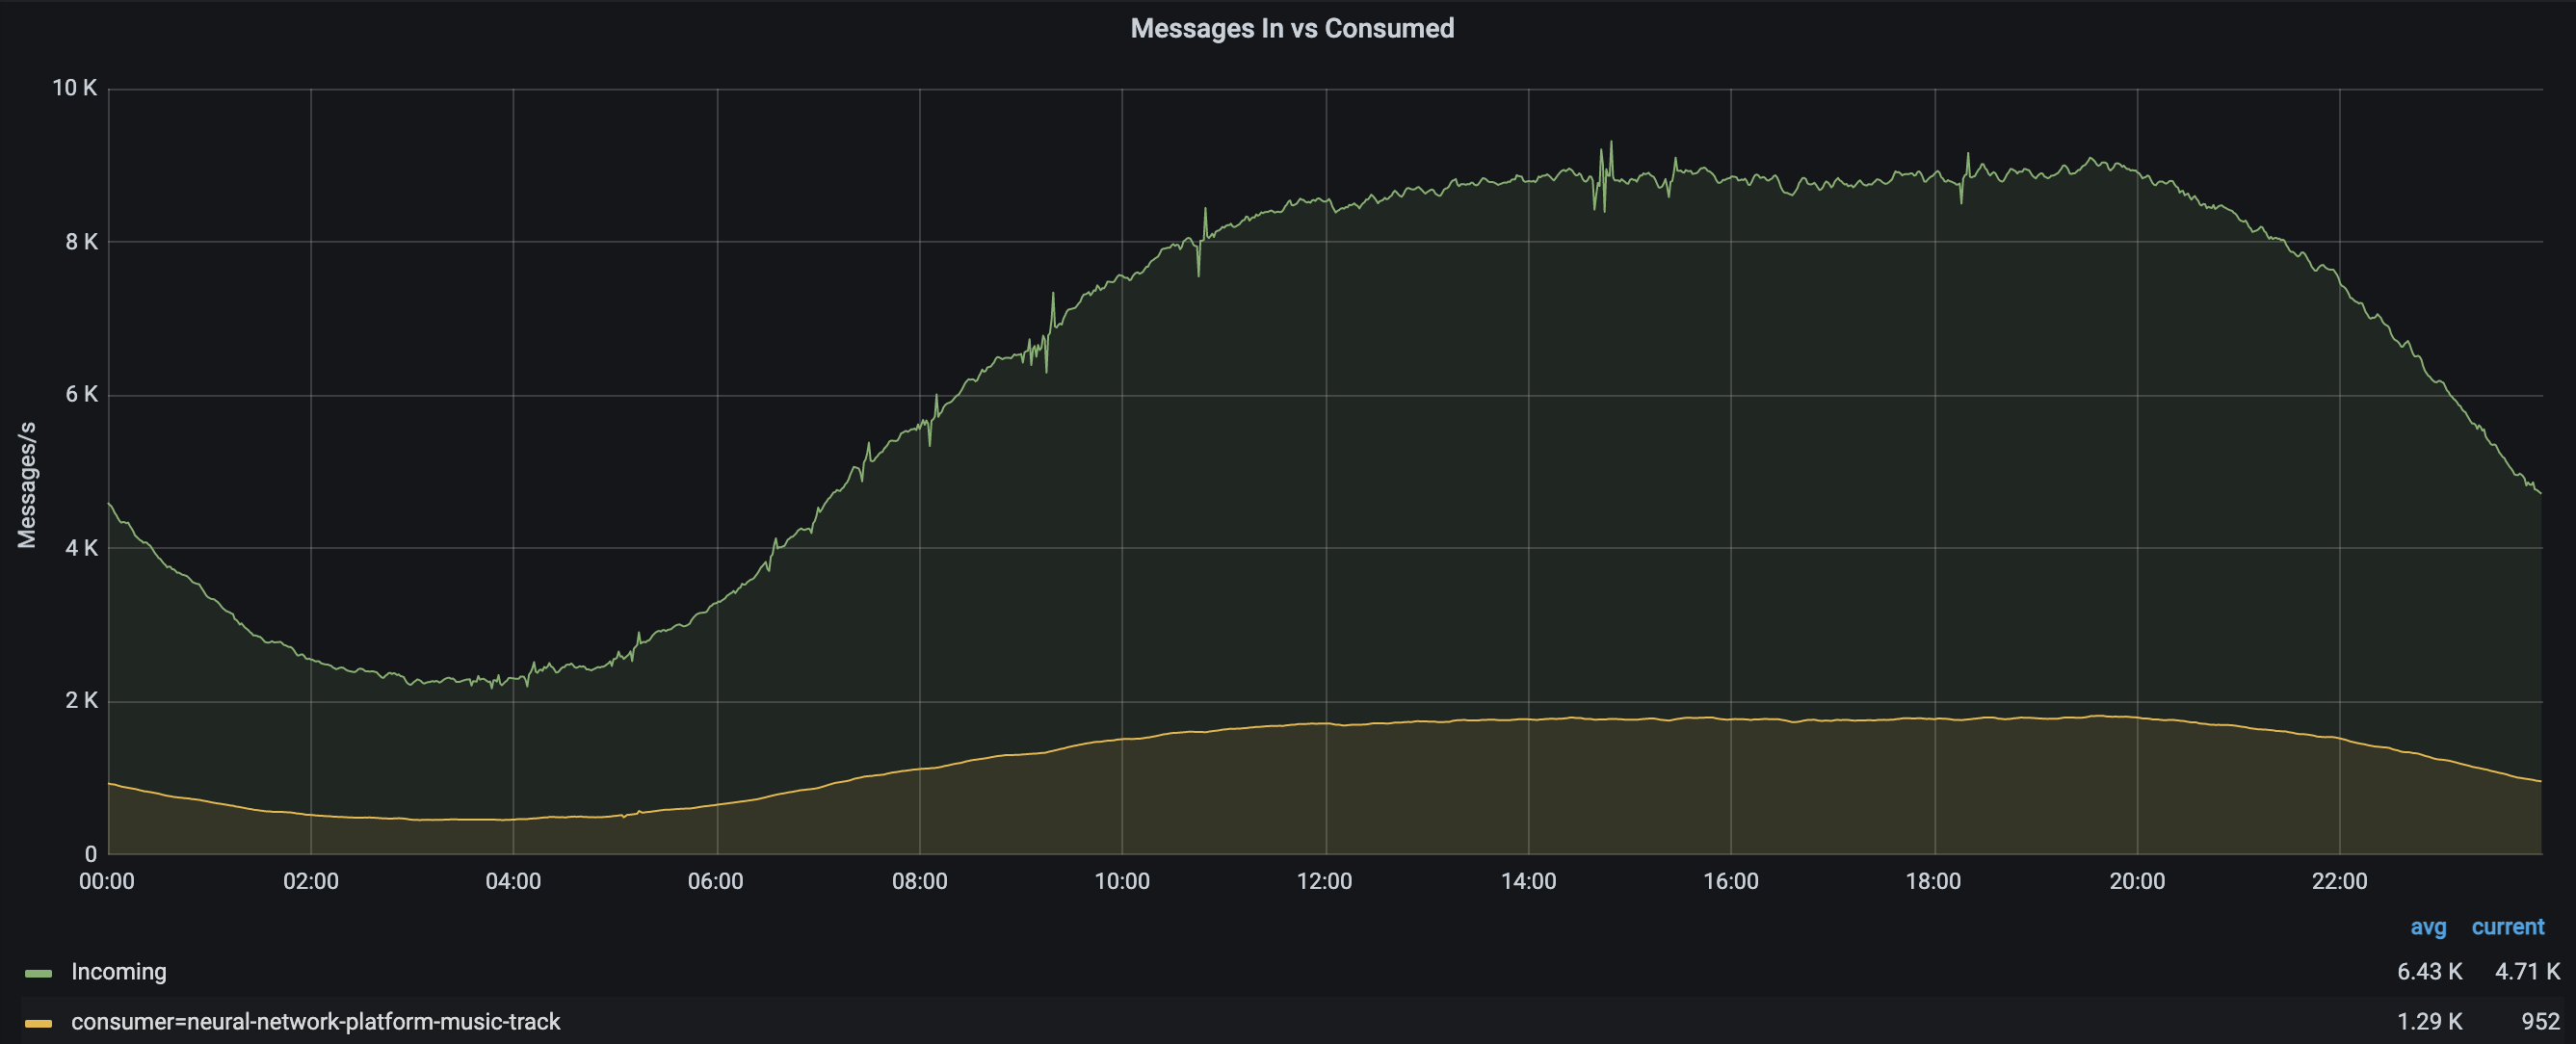
\includegraphics[scale=0.25]{images/music-activity.png}
\end{center}

\begin{itemize}[<+->]
\vkitem Хранение данных для анализа
\vkitem Потоковая обработка данных (Spark Streaming, Apache Samza)
\end{itemize}

\end{frame}

\begin{frame}{Хранение и анализ данных}

\begin{center}
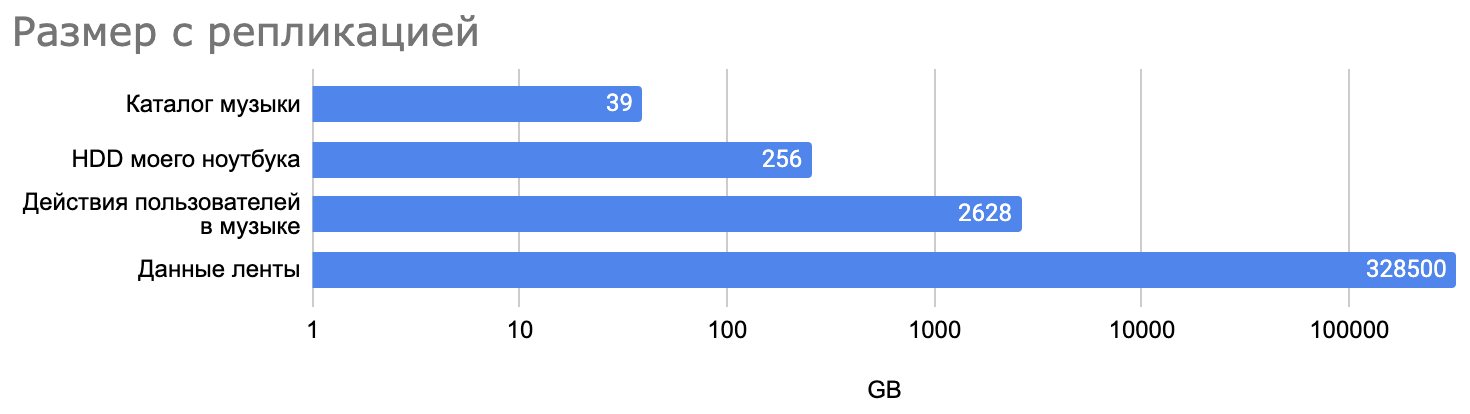
\includegraphics[scale=0.5]{images/data-size.png}
\end{center}

\pause

\begin{itemize}[<+->]
\vkitem Распределенная файловая система: Hadoop HDFS
\vkitem Анализ данных: Apache Spark
\vkitem Контроль выполнения: Apache Airflow
\end{itemize}

\end{frame}

\begin{frame}{}

\begin{center}
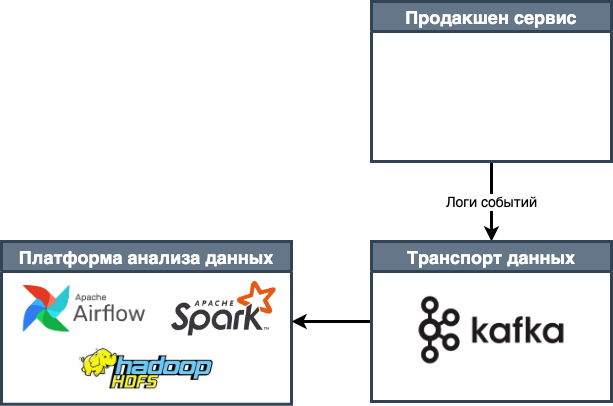
\includegraphics[scale=0.35]{images/bigdata.png}
\end{center}

\end{frame}

{
\usebackgroundtemplate{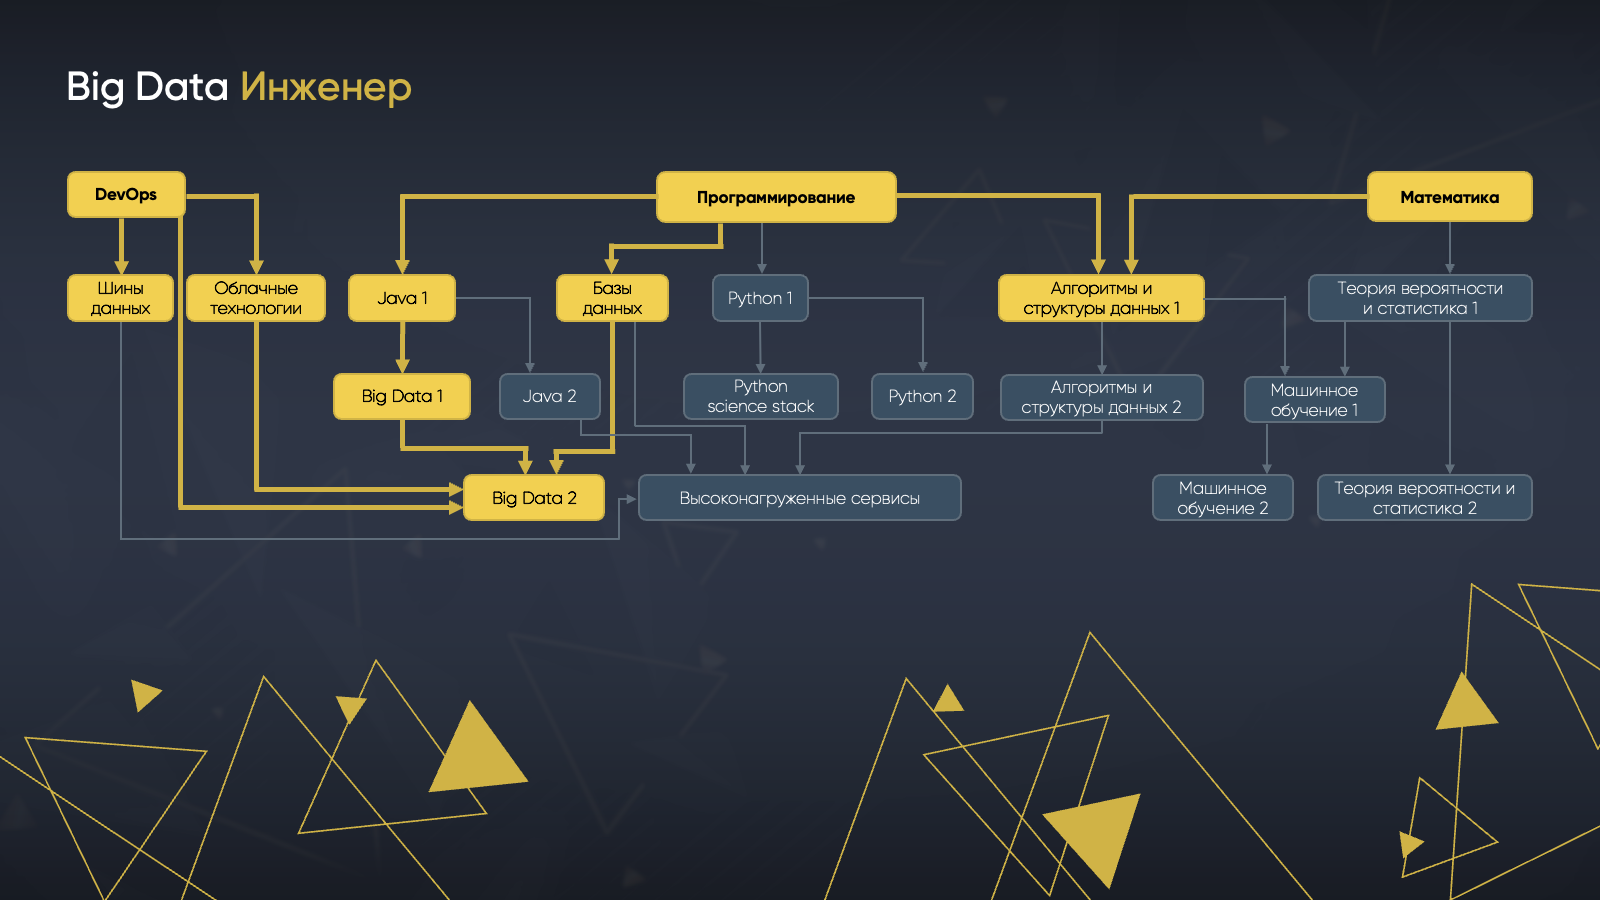
\includegraphics[width=\paperwidth]{images/bde.png}}
\begin{frame}[plain]
\end{frame}
}

\section{Наука о рекомендациях}

{
\usebackgroundtemplate{
\includegraphics[width=\paperwidth]{images/part-4.png}}
\begin{frame}[plain]
\end{frame}
}

\begin{frame}{Количество статей с ``recommender system'' в названии}
\begin{center}
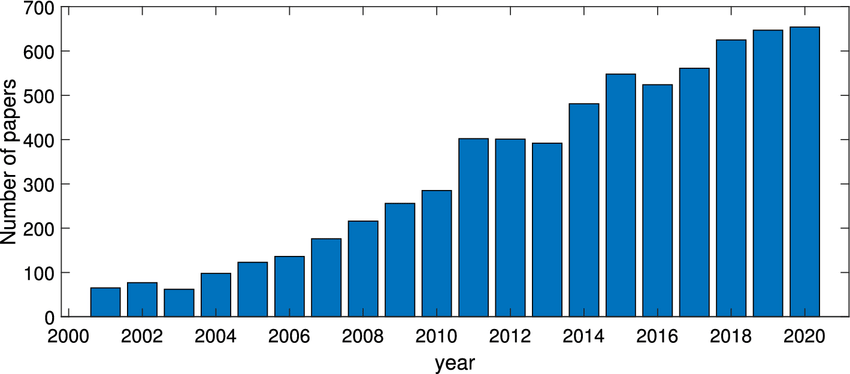
\includegraphics[scale=1.5]{images/publications.png}
\end{center}
\end{frame}

\begin{frame}{Актуальные задачи в науке о рекомендациях}

\begin{columns}

\begin{column}{0.5\textwidth}
\begin{itemize}[<+->]
\vkitem Новые алгоритмы
\vkitem Счастье пользователей
	\begin{itemize}
	\vkitem Долгосрочный эффект
	\vkitem Многосторонние маректплейсы
	\vkitem Честность рекомендаций
	\end{itemize}
\item Выйти из пузыря
	\begin{itemize}
	\vkitem Разнообразие рекомендаций
	\vkitem Reinforcement learning
	\end{itemize}
\item Пользовательский опыт
	\begin{itemize}
	\vkitem Объяснения рекомендаций
	\vkitem Настройки рекомендаций
	\vkitem Оптимизация UI
	\end{itemize}
\end{itemize}
\end{column}

\begin{column}{0.4\textwidth}
\begin{center}

\includegraphics[scale=0.2]{images/science.jpeg}
\end{center}
\end{column}

\end{columns}

\end{frame}

{
\usebackgroundtemplate{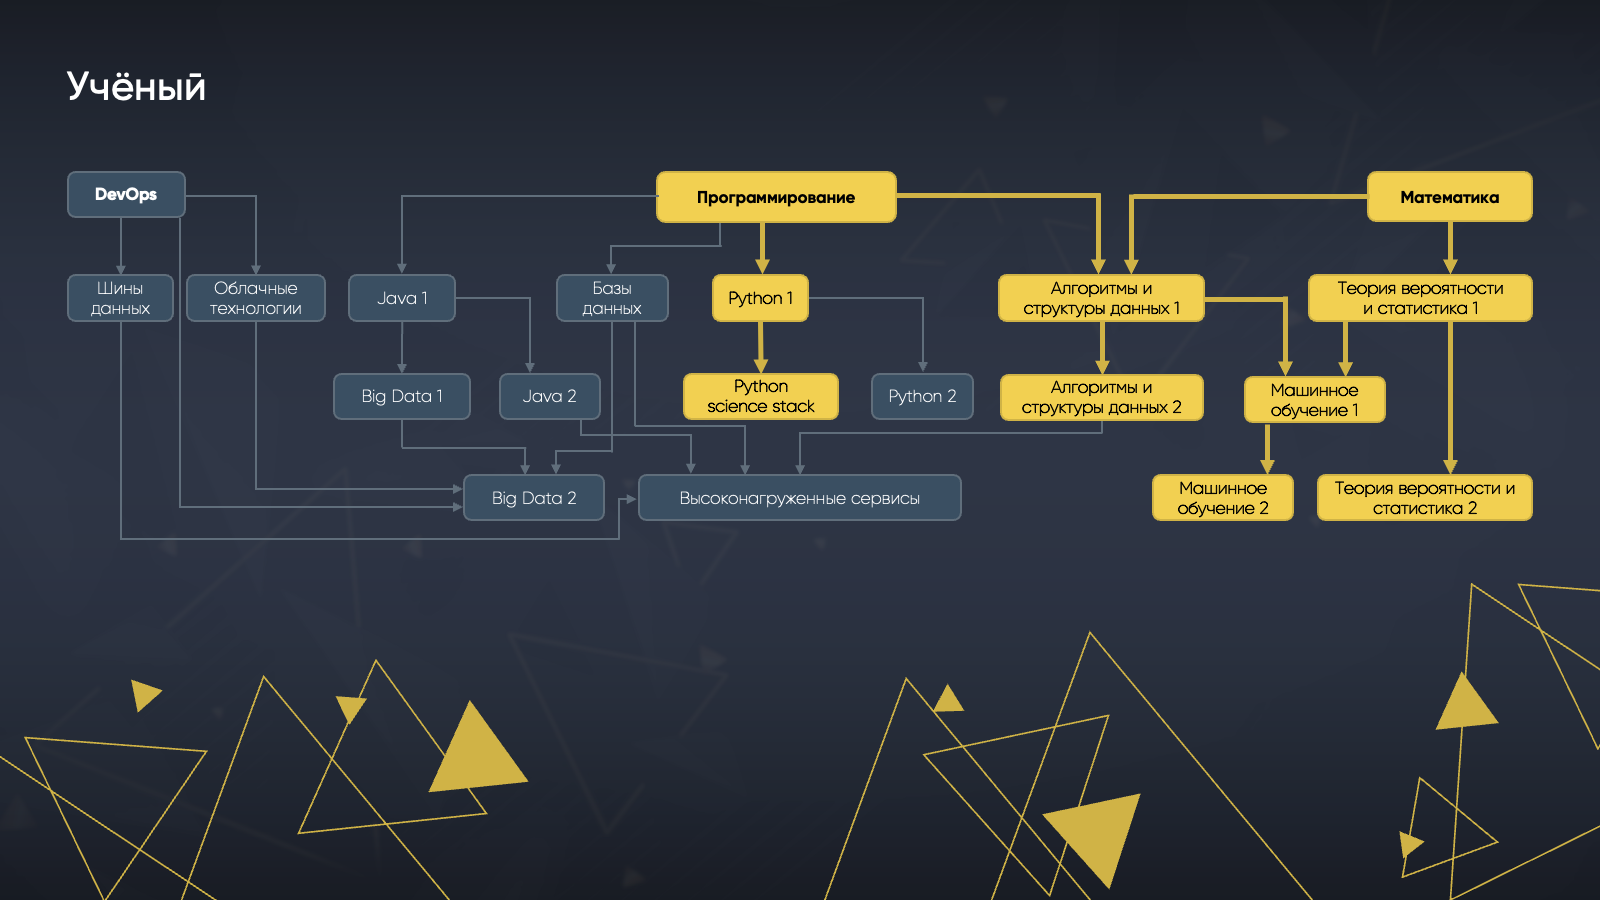
\includegraphics[width=\paperwidth]{images/sci.png}}
\begin{frame}[plain]
\end{frame}
}

\section{Итоги}

{
\usebackgroundtemplate{
\includegraphics[width=\paperwidth]{images/conclusion.png}}
\begin{frame}[plain]
\end{frame}
}

\begin{frame}{Готовая рекомендательная система}
\begin{center}
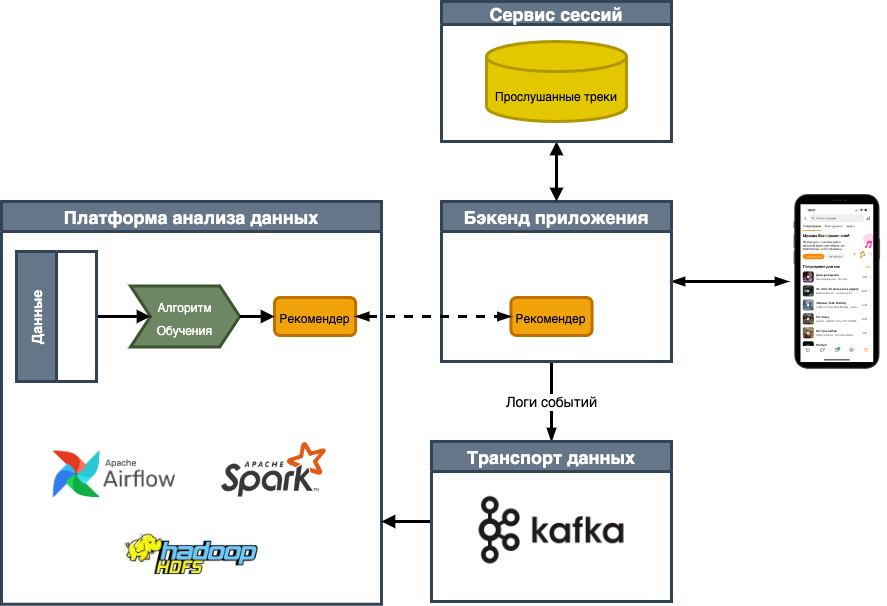
\includegraphics[scale=0.3]{images/architecture.png}
\end{center}
\end{frame}

{
\usebackgroundtemplate{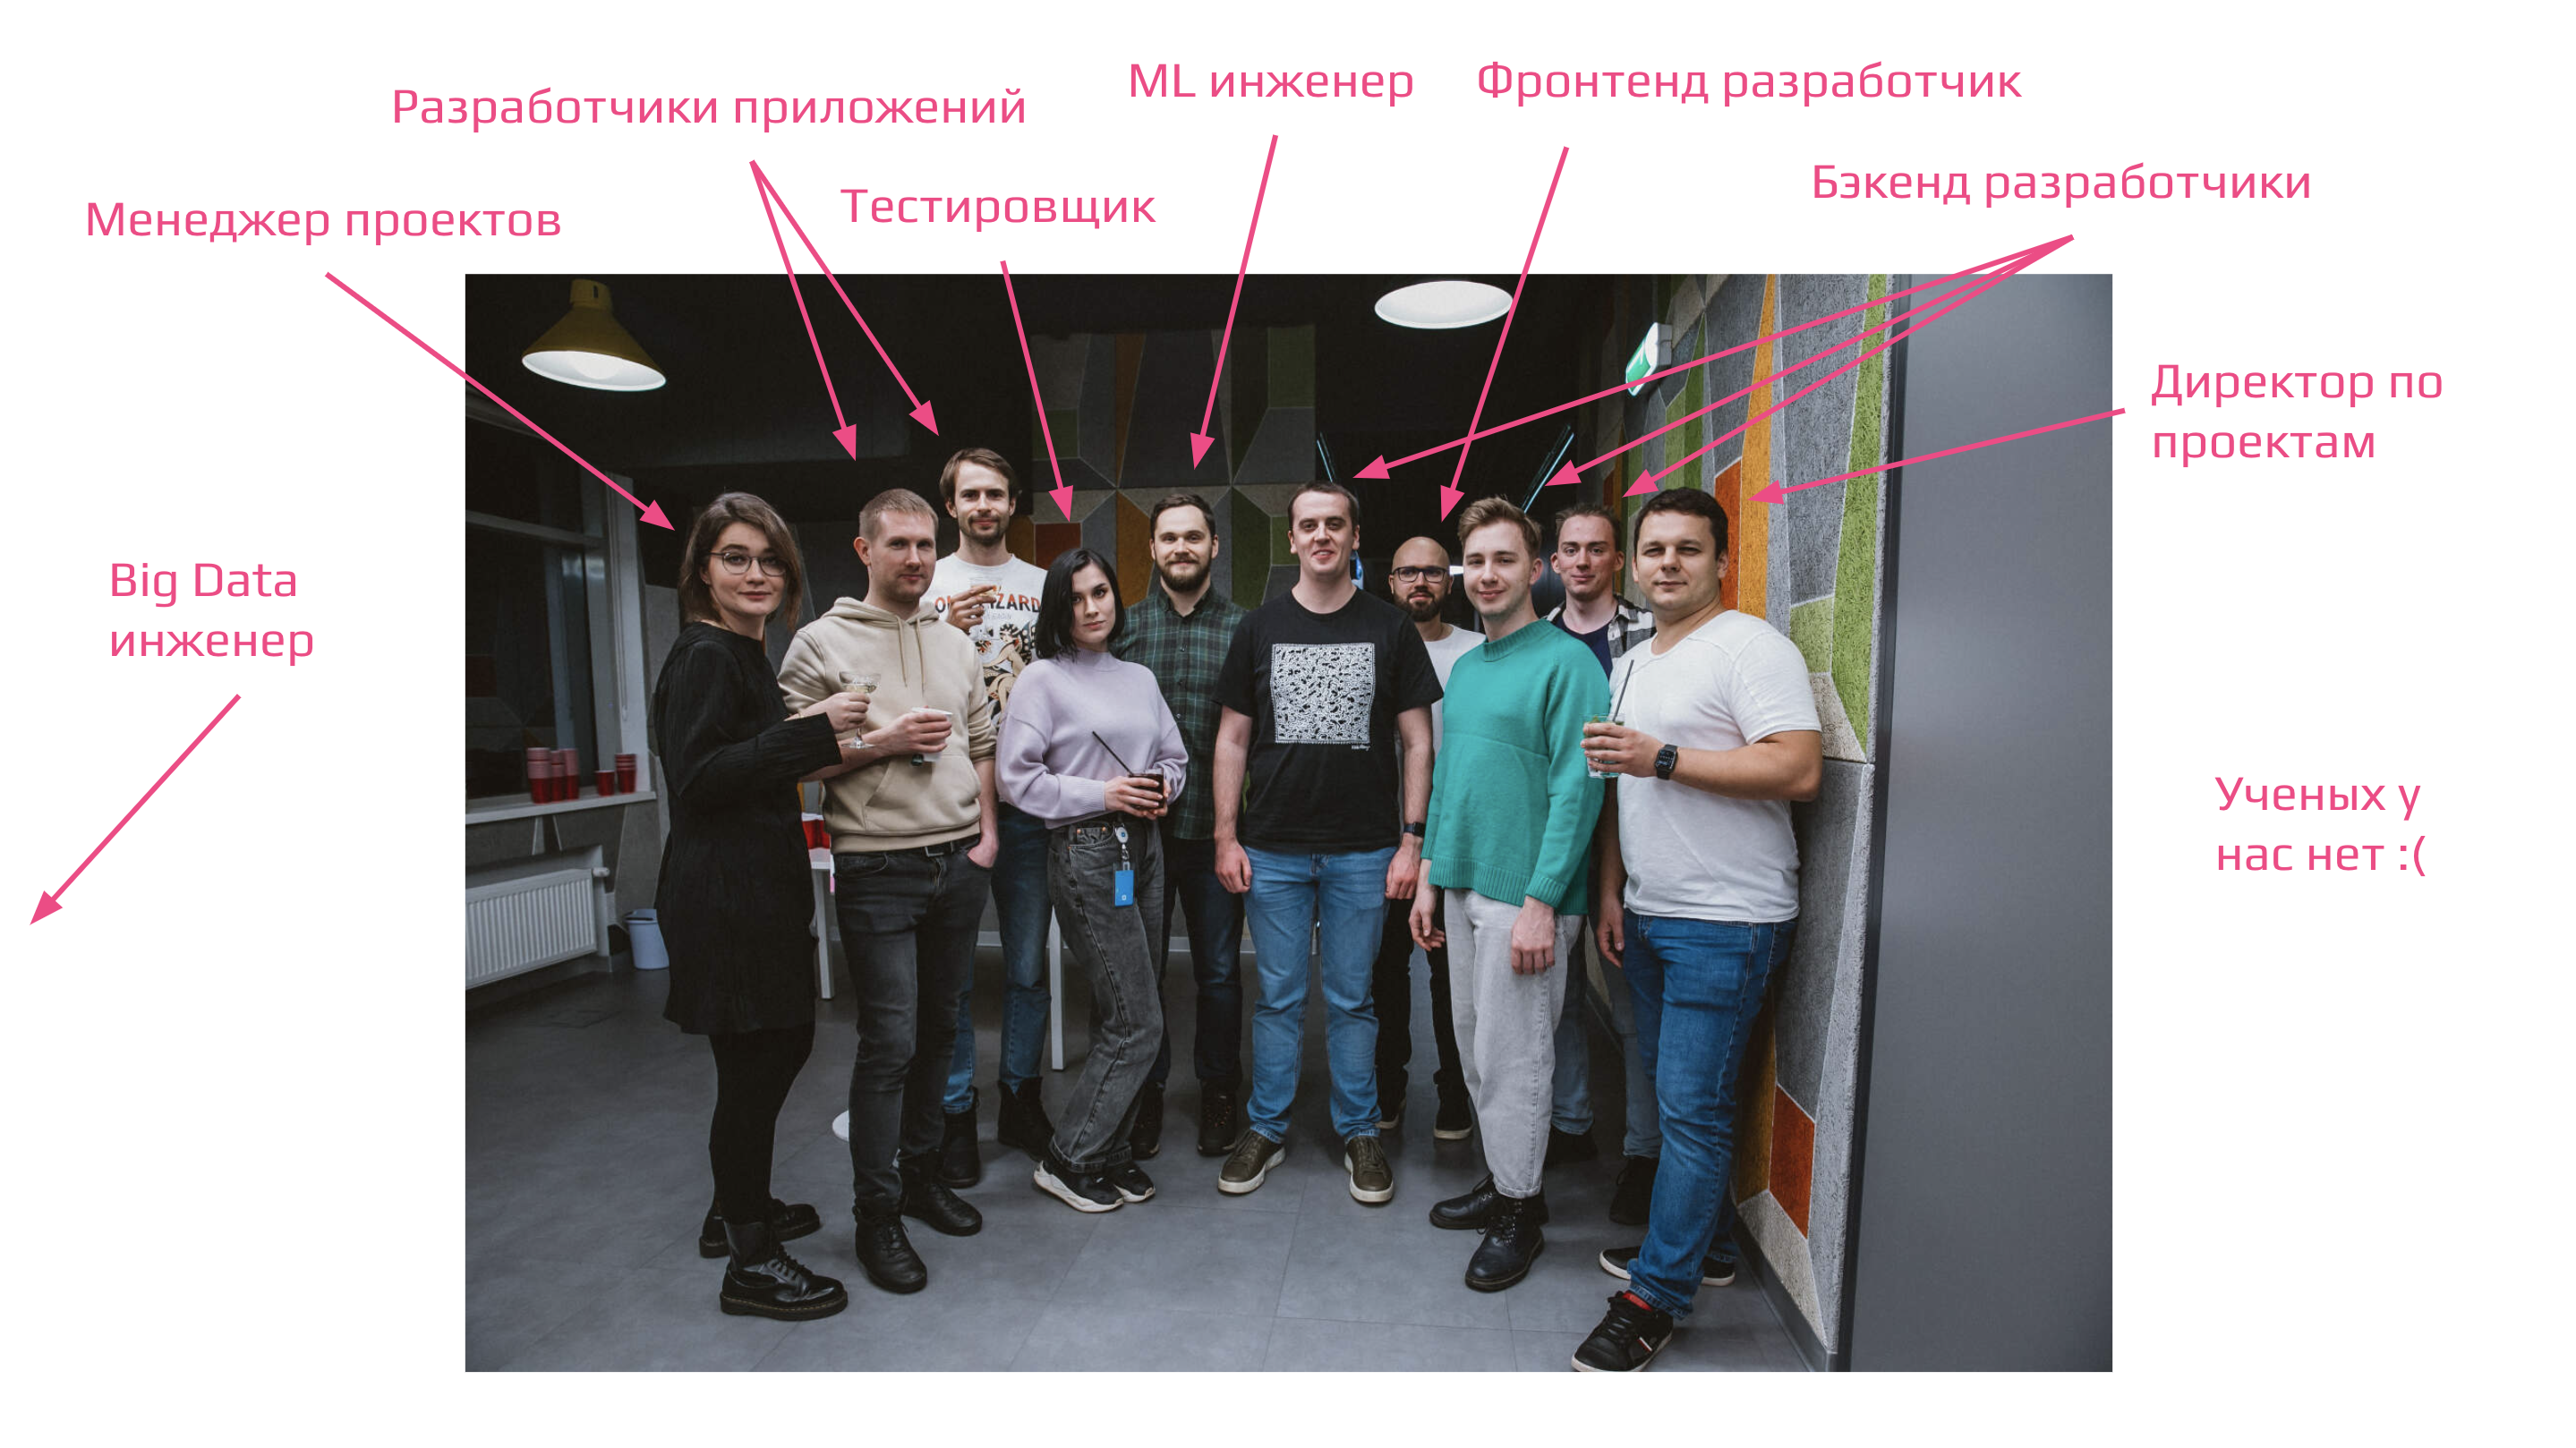
\includegraphics[width=\paperwidth]{images/team.png}}
\begin{frame}[plain]
\end{frame}
}

{
\usebackgroundtemplate{
\includegraphics[width=\paperwidth, height=\paperheight]{images/thankyou.png}}
\begin{frame}[plain]
\end{frame}
}

\begin{frame}[allowframebreaks]{Литература}
\bibliographystyle{amsalpha}
\bibliography{references.bib}
\end{frame}

\end{document}
